\documentclass[a4paper,12pt,twoside]{article}
\usepackage[left=1in,right=1in,top=1in,bottom=1in]{geometry}

\usepackage{xeCJK}
\setCJKmainfont{Songti TC}
\setCJKfamilyfont{kai}{Songti TC}
\newcommand{\kai}{\CJKfamily{kai}} % 用 \kai{使用楷書}

\usepackage{lmodern}
\usepackage{titling}
\usepackage{titlesec}
\usepackage{graphicx}
\usepackage{float}
\usepackage{amsmath, amsthm, amssymb, amsfonts, mathrsfs}
\usepackage{upgreek} % 直立的希臘字母

\usepackage[shortlabels]{enumitem}
\usepackage{setspace}
\renewcommand{\baselinestretch}{1.5}
\usepackage[colorlinks]{hyperref}
\usepackage{fancyvrb}
\usepackage{fancyhdr}
\usepackage{multicol}
\usepackage{caption}
\usepackage{listings}
\usepackage{bm}
\usepackage{bbm} % for \mathbbm{1} (indicator function)
\usepackage{centernot}
\usepackage{mdframed}
\usepackage{tikz}
\usetikzlibrary{patterns, arrows.meta, positioning}
\usepackage[nameinlink, capitalise]{cleveref}
\usepackage{diagbox}
\usepackage{booktabs}
\usepackage{multirow,array}
\usepackage{tabularx}
\usepackage{mathtools}
\usepackage{indentfirst} % 首段 indent
\setlength{\parindent}{2em}
\usepackage{cancel} % 數學式子畫線槓掉
\newcommand\mcancel[2][red]{\setbox0=\hbox{$#2$}%
\rlap{\raisebox{.45\ht0}{\textcolor{#1}{\rule{\wd0}{1pt}}}}#2}
\usepackage{datetime2}

\AtBeginDocument{%
 \setlength{\abovedisplayskip}{6pt}
 \setlength{\belowdisplayskip}{6pt}
 \setlength{\abovedisplayshortskip}{4pt}
 \setlength{\belowdisplayshortskip}{4pt}
}

\definecolor{codegreen}{rgb}{0,0.6,0}
\definecolor{codegray}{rgb}{0.5,0.5,0.5}
\definecolor{codepurple}{rgb}{0.58,0,0.82}
\definecolor{backcolour}{rgb}{0.95,0.95,0.92}

\lstdefinestyle{mystyle}{
 backgroundcolor=\color{backcolour},
 commentstyle=\color{codegreen},
 keywordstyle=\color{magenta},
 numberstyle=\tiny\color{codegray},
 stringstyle=\color{codepurple},
 basicstyle=\ttfamily\footnotesize,
 breakatwhitespace=false,
 breaklines=true,
 captionpos=b,
 keepspaces=true,
 numbers=left,
 numbersep=5pt,
 showspaces=false,
 showstringspaces=false,
 showtabs=false,
 tabsize=2
}
\lstset{style=mystyle}

\hypersetup{citecolor=blue, linkcolor=blue, urlcolor=blue}

\DeclareMathOperator{\supp}{supp}
\DeclareMathOperator{\skewness}{Skewness}
\DeclareMathOperator{\DU}{D-U}
\DeclareMathOperator{\CU}{C-U}
\DeclareMathOperator{\Geo}{Geo}
\DeclareMathOperator{\Pois}{Pois}
\DeclareMathOperator{\Gam}{Gam}
\DeclareMathOperator{\LN}{LogN}
\DeclareMathOperator{\cov}{Cov}
\DeclareMathOperator*{\argmax}{arg\,max}
\DeclareMathOperator*{\argmin}{arg\,min}
\DeclareMathOperator{\re}{Re}
\DeclareMathOperator{\im}{Im}

\newcommand{\N}{\mathbb{N}}
\newcommand{\Z}{\mathbb{Z}}
\newcommand{\Q}{\mathbb{Q}}
\newcommand{\R}{\mathbb{R}}
\newcommand{\C}{\mathbb{C}}
\newcommand{\G}{\mathcal{G}}
\newcommand{\mP}{\mathbb{P}}
\newcommand{\F}{\mathcal{F}}
\newcommand{\B}{\mathcal{B}}
\newcommand{\1}{\mathbbm{1}}
\newcommand{\Poi}{\text{Poi}}
\newcommand{\Var}{\text{Var}}
\newcommand{\as}{\text{a.s.}}
\newcommand{\vect}[1]{\boldsymbol{\mathbf{#1}}}
\newcommand{\paren}[1]{\left({#1}\right)}
\newcommand{\brk}[1]{\left[{#1}\right]}
\newcommand{\curl}[1]{\left\{{#1}\right\}}
\renewcommand{\lambda}{\lambdaup}

\theoremstyle{definition} % 定理環境 style 改用正體
\newtheorem{theorem}{定理}
\newtheorem{definition}{定義}
\newtheorem*{definition*}{定義}
\newtheorem{example}{例子}
\newtheorem{exercise}{練習}
\newtheorem{corollary}{推論}
\newtheorem{property}{性質}
\newtheorem{prop}{命題}
\newtheorem{lemma}{引理}
\newtheorem{problem}{問題}
\newtheorem*{remark}{註}

\renewcommand{\figurename}{圖}
\renewcommand{\tablename}{表}

\DeclareMathOperator{\var}{Var}
\DeclareMathOperator{\corr}{corr}
\DeclareMathOperator{\rank}{rank}
\DeclareMathOperator{\MSE}{MSE}
\DeclareMathOperator{\SSE}{SSE}
\DeclareMathOperator{\SST}{SST}
\DeclareMathOperator{\SSR}{SSR}
\DeclareMathOperator{\sgn}{sign}
\DeclareMathOperator{\alt}{Alt}
\DeclareMathOperator{\adj}{adj}
\DeclareMathOperator{\curlOp}{curl}
\DeclareMathOperator{\spn}{span}
\DeclareMathOperator{\sse}{SSE}
\DeclareMathOperator{\tr}{tr}

\newcommand{\ep}{\varepsilon}
\newcommand{\p}{\partial}
\newcommand{\abs}[1]{\left|#1\right|}
\newcommand\norm[1]{\left\lVert#1\right\rVert}
\newcommand{\innerprod}[1]{\langle#1\rangle}
\newcommand{\ds}{\displaystyle}
\newcommand{\blank}{\rule[-1mm]{1.5cm}{0.1mm}}
\newcommand{\dint}{\displaystyle\int}
\renewcommand{\bar}{\overline}

\newtheoremstyle{remark}{}{}{}{}{\bfseries\sffamily}{.}{.5em}{#1}
\theoremstyle{remark}

\newtheorem*{remark*}{\textit{Remark}}
\newtheorem*{solution*}{解}

\AtEndEnvironment{solution*}{\hfill$\square$}
\newtheorem*{hint*}{Hint}


\usepackage{tcolorbox}
\tcbuselibrary{skins,breakable}
\usetikzlibrary{patterns,decorations.pathreplacing,decorations.markings,decorations.shapes,decorations.pathmorphing,calc,3d}

\newenvironment{example-non}[1][]{\vspace{0.8em}\noindent\textbf{#1}\quad}{\vspace{0.8em}}
\newenvironment{solution}{\par\noindent\textbf{解}\quad}{\par\vspace{0.8em}}

\newcommand{\redtext}[1]{{\color{red} #1}}
\newcommand{\bluetext}[1]{{\color{blue} #1}}

\fancypagestyle{firstpage}{
  \fancyhf{}
  \fancyhead[R]{\small《高中數學實驗教材》第 4 冊（自然組）}
  \fancyhead[L]{\small 第 5 章\quad 複數與三角基本定理}
  \fancyfoot[C]{\thepage}
}

\pagestyle{fancy}
\setlength{\headheight}{14pt}
\renewcommand{\headrulewidth}{0.5pt}
\renewcommand{\footrulewidth}{0pt}
\fancyhead{}
\fancyhead[LE]{\small 《高中數學實驗教材》第四冊（自然組）}
\fancyhead[RO]{\small 第五章\quad 複數與三角基本定理}
\fancyfoot[C]{\thepage}

\title{\LARGE\textbf{《高中數學實驗教材》第四冊（自然組）}\\[0.5em] \Large\textbf{第五章\quad 複數與三角基本定理}}
\author{\textbf{高中數學實驗教材編輯小組}\quad 編著}
\date{民國六十五年（1976）三版}

\begin{document}

\maketitle
\thispagestyle{firstpage}

% ==========================================
% 掃描檔勘誤、文字校訂與疑難處說明（依規則整理於目錄之前）
% ==========================================
\section*{【說明】第五章掃描檔勘誤、疑難處與文義校訂表}
\addcontentsline{toc}{section}{【說明】第五章掃描檔勘誤、疑難處與文義校訂表}

本章數位化轉錄依據 1976 年版原書掃描檔案進行逐字、逐式忠實校錄．對原書中因早期鉛字印刷、手工排版所致之訛字、衍字、倒裝、脫漏及圖形標註微瑕，均本於「字符級忠實度」與「嚴謹學術校訂」原則，於正文完整保留原貌並以註腳精確標註，彙整校訂說明如下：

\begin{table}[htbp]
\centering
\small
\begin{tabularx}{\textwidth}{|c|p{4.2cm}|p{4.5cm}|X|}
\hline
\textbf{頁碼} & \textbf{原書印刷／掃描原貌} & \textbf{數位校訂／規範化形式} & \textbf{校訂說明與學術理由} \\ \hline
p.256 & 倒數第 8 行原印 $(3+i)\cdot(1+2i) = 3-6i+\dots$ & $(3+i)\cdot(1-2i) = 3-6i+i-2i^2 = 5-5i$ & 原書第二因式誤植為加號，依展開式與文義校訂為減號 $(1-2i)$． \\ \hline
p.259 & 倒數第 7 行原印 $x=0, y=\sqrt{-a}$ & $x=0, y=\pm\sqrt{-a}$ & 解方程式 $y^2 = -a$ 應有正負二根，補正 $\pm$． \\ \hline
p.261 & 習題 V-1 第 4 題漏編 (iv) 直跳 (v) & 保留原編號 (i), (ii), (iii), (v) & 忠實保留原書題號編排，加註說明原書漏編 (iv)． \\ \hline
p.267 & 例 6 原書計算式行距較緊湊 & 排版優化並保持公式完整 & 保留共軛複數與長度性質之原始推導過程． \\ \hline
p.286 & 習題 V-3 第 11(i) 題誤印 $\frac{1}{2}$ & $\sin^4\theta = \frac{1}{8}\cos 4\theta - \frac{1}{2}\cos 2\theta + \frac{3}{8}$ 或 $\frac{1}{4}$ 關係 & 原書係數印刷微瑕，依三角展開公式校訂補註． \\ \hline
p.287 & ‡§ V-4 里曼球面符號 ${}^\ddagger$ & 保留 ${}^\ddagger$ 標記 & 表示雙重星號等級之進階選修教材，忠實呈現原書標示． \\ \hline
p.297 & 習題 V-5 獨立題組 & § V-4 丙「球的轉動」後獨立設「習題 V-5」 & 原書在 § V-4 內編排兩套習題（習題 V-4 與 V-5），忠實完整收錄． \\ \hline
\end{tabularx}
\end{table}

\vspace{1em}
\hrule
\vspace{1em}

\tableofcontents
\newpage

% =========================================================================
% 《高中數學實驗教材》第四冊（自然組）
% 第五章 複數與三角基本定理
% =========================================================================

\section{複數與三角基本定理}
\label{sec:b4-ch5}

\begin{center}
\begin{minipage}{0.75\textwidth}
\begin{itemize}[leftmargin=2em, itemsep=0.3em]
  \item[§ V-1] \textbf{複數系的基本性質}
  \begin{itemize}[leftmargin=2em, itemsep=0.2em]
    \item[甲、] 複數系的建立
    \item[乙、] 複數系的基本性質
  \end{itemize}
  \item[§ V-2] \textbf{平面的複數坐標系——高斯平面}
  \begin{itemize}[leftmargin=2em, itemsep=0.2em]
    \item[甲、] 平面複數坐標系
    \item[乙、] 平面上的向量與複數
    \item[丙、] 複數乘法與複角公式
    \item[丁、] $n$ 次方根
    \item[戊、] 共軛與$^*$鏡射
  \end{itemize}
  \item[§ V-3] \textbf{三角恆等式及三角恆等式基本定理}
  \begin{itemize}[leftmargin=2em, itemsep=0.2em]
    \item[甲、] 基本三角恆等式
    \item[乙、] 一些常用的三角恆等式
    \item[丙、] 三角恆等式基本定理
  \end{itemize}
  \item[${}^\ddagger$§ V-4] \textbf{里曼球面}
  \begin{itemize}[leftmargin=2em, itemsep=0.2em]
    \item[甲、] 球面投影
    \item[$^*$乙、] 球面映射與平面映射的對應
    \item[$^{**}$丙、] 球的轉動
  \end{itemize}
\end{itemize}
\end{minipage}
\end{center}

\begin{center}
$* \qquad * \qquad * \qquad * \qquad *$
\end{center}

在討論長度，面積，體積，質量等等的度量的過程中，自然地產生了實數系這個最基本，最有用的數學體系．在本書的第一冊及第二冊中，我們由最簡單的整數系出發，逐步漸進地經由有理數系，對於實數系在運算上與極限上的種種簡潔有用的性質，做了一次有系統的介紹與討論．一般說來，實數系是一個相當完備而優良的體系；對於各種實用問題，極大部分都可以在實數系裏有效而簡明地予以解決．但是對於某些問題，實數系依然有不夠完備的地方．譬如我們在第二冊第一章所討論的二次方程式中，如果 $b^2-4ac < 0$，那麼方程式 $ax^2+bx+c=0$ 在實數系中無解，一個最簡單的情形就是 $x^2+1=0$ 無實數解．

對於實數系在這方面的欠缺的補救辦法，是在實數系之外，另創一個新數 $i$，叫做\textbf{虛數單位}，滿足 $i^2=-1$（也就是說 $i$ 是 $x^2+1=0$ 的解）．然後由實數與 $i$ 作成新數，稱為\textbf{複數}；實數系經過這樣的擴充而得的數系，就是\textbf{複數系}．換句話說，複數系是由實數系經過適當的擴充而得到的數系．它比實數系更加完備，所以在若干問題的討論上，複數系用起來要比實數系更簡捷，更有效．

負數的平方根早在十六世紀即已有人討論，而虛數單位 $i$ 則係由歐拉（Euler 1707--1783）首先採用．複數的觀念最初並不能為一般人所接受，因為在應用時尚未遇到過用複數表示的量．其後高斯（Gauss 1777--1855）將複數用平面上的點來表示，使得大家對於複數有了進一步的認識．並且由於數學的發展，確認數系就是一種具有加，乘兩種運算，滿足若干基本性質的體系．這樣，複數系才得到它在數學中應有的地位．另一方面，在若干應用問題（如力學，電學等）中亦已發現若干要用複數才能適當表示的量．

在本章中將討論複數系的基本性質，高斯平面以及複數與三角函數的關係．


\subsection{§ V-1\texorpdfstring{\quad }{ }複數系的基本性質}

\subsubsection*{甲、複數系的建立}

對於任意 $x \in \mathbf{R}$，我們都有
\[
x^2 \ge 0 \implies x^2+1 \ge 1.
\]
因此方程式 $x^2+1=0$ 不可能有實數解．現在我們用下列基本關係
\[
i^2 = -1
\]
定義一個不屬於 $\mathbf{R}$ 的新數 $i$，叫做\textbf{虛數單位}．則 $i$ 即滿足方程式 $x^2+1=0$．

其次我們用實數與 $i$ 作成下列形式的數
\[
a+bi, \quad a, b \in \mathbf{R},
\]
叫做\textbf{複數}，而把 $a$ 叫做複數 $a+bi$ 的\textbf{實部}，$b$ 叫做\textbf{虛部}．當虛部 $b=0$ 時，就寫為 $a+0i=a$；也就是說，把一般的實數 $a$ 看作虛部為 $0$ 的複數．當實部 $a=0$ 時，就寫為 $0+bi=bi$，叫做\textbf{虛數}（或\textbf{純虛數}）；換句話說，虛數就是實部為 $0$ 的複數．既是實數又是虛數的複數只有 $0$ 一個：
\[
0 = 0+0i = 0i.
\]
所有複數所成的集合
\[
\{a+bi \mid a, b \in \mathbf{R}\}
\]
附上以下所定義的加，乘運算，就成為一個數系，叫做\textbf{複數系}，記為 $\mathbf{C}$．根據以上的約定以及以前各種數系的擴展關係，我們有
\[
\begin{matrix}
\mathbf{N} & \subsetneq & \mathbf{Z} & \subsetneq & \mathbf{Q} & \subsetneq & \mathbf{R} & \subsetneq & \mathbf{C} \\
\text{（自然數系）} & & \text{（整數系）} & & \text{（有理數系）} & & \text{（實數系）} & & \text{（複數系）}
\end{matrix}
\]

現在我們要來定義複數系上的加法與乘法運算，我們要求所定義的運算，還能保持實數系原有的基本性質，如交換律，結合律，分配律等等．由於實數系上多項式的加法與乘法運算滿足這些基本性質，我們就規定複數系 $\mathbf{C}$ 上的加，乘運算依照多項式的加，乘規則來演算，但是要顧到 $i$ 的基本關係 $i^2=-1$．也就是說，我們在計算時先把 $i$ 看作不定元，然後再把 $i^2$ 以 $-1$ 代入，例如
\begin{align*}
(3+i)+(1-2i) &= (3+1)+(i-2i) = 4-i, \\
(3+i)\cdot(1-2i) &= 3-6i+i-2i^2 \\
&= 3-5i-2(-1) = 5-5i.
\end{align*}
\phantomsection\label{note:b4-ch5-p256-errata}\footnote{【原書註記/校訂】：原書印為 $(3+i)\cdot(1+2i) = 3-6i+i-2i^2$，由計算展開式及結果可知第二因式實為 $(1-2i)$，正文予以校訂修正．}

根據多項式的運算，我們首先推出下列簡單的關係：

設 $a+bi, a'+b'i \in \mathbf{C}$ ($a, b, a', b' \in \mathbf{R}$)，則
\begin{itemize}
  \item[(i)] $a+bi = a'+b'i \iff a=a' \text{ 及 } b=b'$． \\
  這就是說，二複數相等即其實部與虛部分別相等．
  \item[(ii)] $(a+bi)+(a'+b'i) = (a+a')+(b+b')i$． \\
  這就是說，二複數相加即其實部與虛部分別相加．
  \item[(iii)] $(a+bi)\cdot(a'+b'i) = (aa'-bb')+(ab'+a'b)i$． \\
  這個公式可用於求複數的積，由下列計算得到：
  \begin{align*}
  (a+bi)(a'+b'i) &= aa'+ab'i+ba'i+bb'i^2 \\
  &= aa'+ab'i+ba'i-bb' \\
  &= (aa'-bb')+(ab'+a'b)i.
  \end{align*}
\end{itemize}

\subsubsection*{作業 1}
求滿足下列各式的實數 $x, y$：
\begin{itemize}
  \item[(i)] $(x+yi)+(7-3i) = 5+2i$
  \item[(ii)] $2x+yi = 1+(3+5i)$
  \item[(iii)] $(x+yi)-(4+2i) = 6-8i$
\end{itemize}


\noindent〔註〕對於複數系的建立，我們也可以不考慮基本關係 $i^2=-1$，而把 $i$ 純粹看作一個符號，再用上面的 (i) 至 (iii) 作為複數相等，相加，相乘的定義．那時候我們就可以由 (iii) 式導出 $i^2=-1$．

\subsubsection*{乙、複數系的基本性質}

設 $c_1 = a_1+b_1i, c_2 = a_2+b_2i, c_3 = a_3+b_3i \in \mathbf{C}$，則由上述複數的加法與乘法公式 (ii) 及 (iii)，可以驗證下列加，乘運算所具有的基本性質：

\paragraph{I. 交換律：} $c_1+c_2 = c_2+c_1, \quad c_1\cdot c_2 = c_2\cdot c_1$．
\begin{proof}[驗證]
\begin{align*}
c_1+c_2 &= (a_1+b_1i)+(a_2+b_2i) \\
&= (a_1+a_2)+(b_1+b_2)i && \text{〔由 (ii)〕} \\
&= (a_2+a_1)+(b_2+b_1)i && \text{〔實數加法交換律〕} \\
&= (a_2+b_2i)+(a_1+b_1i) && \text{〔由 (ii)〕} \\
&= c_2+c_1.
\end{align*}
\begin{align*}
c_1\cdot c_2 &= (a_1+b_1i)(a_2+b_2i) \\
&= (a_1a_2-b_1b_2)+(a_1b_2+a_2b_1)i && \text{〔由 (iii)〕} \\
&= (a_2a_1-b_2b_1)+(a_2b_1+a_1b_2)i && \text{〔實數交換律〕} \\
&= (a_2+b_2i)(a_1+b_1i) && \text{〔由 (iii)〕} \\
&= c_2\cdot c_1. \qedhere
\end{align*}
\end{proof}

\paragraph{II. 結合律：} $(c_1+c_2)+c_3 = c_1+(c_2+c_3), \quad (c_1c_2)c_3 = c_1(c_2c_3)$．
\begin{proof}[驗證]
加法結合律的驗證比較簡單，我們來驗證乘法結合律．
\begin{align*}
(c_1c_2)c_3 &= [(a_1+b_1i)(a_2+b_2i)](a_3+b_3i) \\
&= [(a_1a_2-b_1b_2)+(a_1b_2+a_2b_1)i](a_3+b_3i) \\
&= [(a_1a_2-b_1b_2)a_3-(a_1b_2+a_2b_1)b_3] \\
&\quad + [(a_1a_2-b_1b_2)b_3+(a_1b_2+a_2b_1)a_3]i \\
&= (a_1a_2a_3-b_1b_2a_3-b_1a_2b_3-a_1b_2b_3) \\
&\quad + (a_1a_2b_3-b_1b_2b_3+a_1b_2a_3+a_2b_1a_3)i,
\end{align*}
\begin{align*}
c_1(c_2c_3) &= (a_1+b_1i)[(a_2+b_2i)(a_3+b_3i)] \\
&= (a_1+b_1i)[(a_2a_3-b_2b_3)+(a_2b_3+a_3b_2)i] \\
&= [a_1(a_2a_3-b_2b_3)-b_1(a_2b_3+a_3b_2)] \\
&\quad + [a_1(a_2b_3+a_3b_2)+b_1(a_2a_3-b_2b_3)]i \\
&= (a_1a_2a_3-a_1b_2b_3-b_1a_2b_3-b_1b_2a_3) \\
&\quad + (a_1a_2b_3+a_1a_3b_2+b_1a_2a_3-b_1b_2b_3)i.
\end{align*}
比較上列二式即得
\[
(c_1c_2)c_3 = c_1(c_2c_3). \qedhere
\]
\end{proof}

\paragraph{III. 分配律：} $c_1(c_2+c_3) = c_1c_2+c_1c_3$．
\begin{proof}[驗證]
留作習題．
\end{proof}

\paragraph{IV. $0$ 與 $1$ 的特性：} 顯然 $0=0+0i$ 是 $\mathbf{C}$ 的零元素，$1=1+0i$ 是 $\mathbf{C}$ 的單位元素：($c \in \mathbf{C}$)
\[
0+c=c+0=c, \quad 0\cdot c = c\cdot 0 = 0;
\]
\[
1\cdot c = c\cdot 1 = c.
\]

\paragraph{V. 可逆性：} 對於任意複數 $c=a+bi \in \mathbf{C}$，存在唯一的元素 $-c \in \mathbf{C}$ 使得
\[
c+(-c)=(-c)+c=0,
\]
不難看出 $-c=(-a)+(-b)i$．對於任給的非零複數 $c=a+bi \neq 0$，存在唯一的倒數 $\frac{1}{c} \in \mathbf{C}$，使得
\[
c\cdot\frac{1}{c} = \frac{1}{c}\cdot c = 1,
\]
由乘法公式 (iii) 可求出
\[
\frac{1}{c} = \frac{a}{a^2+b^2} + \left(\frac{-b}{a^2+b^2}\right)i. \quad \text{（留作習題）}
\]

\begin{example-non}[例 1]
$i$ 的倒數是 $-i$，$-i$ 的倒數是 $i$．
\end{example-non}

\begin{example-non}[論例 1]
設 $c=a+bi \in \mathbf{C}$ 是一個任意給定的複數．試求下列二次方程式的所有複數解：
\[
z^2-c=0.
\]
由此證得任意複數都恰好有兩個平方根．
\end{example-non}

\begin{solution}
設 $z=x+yi$ 滿足上述二次方程式，則有
\[
z^2-c = (x+yi)^2-(a+bi) = (x^2-y^2-a)+(2xy-b)i = 0.
\]
所以 $x, y \in \mathbf{R}$ 滿足下列聯立方程式：
\begin{align}
x^2-y^2 &= a \label{eq:ch5-sec1-1} \\
2xy &= b \label{eq:ch5-sec1-2}
\end{align}
將 \eqref{eq:ch5-sec1-1}, \eqref{eq:ch5-sec1-2} 式兩端平方後相加，得 $(x^2-y^2)^2+(2xy)^2 = a^2+b^2$，化簡得 $(x^2+y^2)^2 = a^2+b^2$．因 $x^2+y^2$ 為正數，故
\begin{equation}
x^2+y^2 = \sqrt{a^2+b^2} \label{eq:ch5-sec1-3}
\end{equation}
由 \eqref{eq:ch5-sec1-1}, \eqref{eq:ch5-sec1-3} 二式解出，亦即
\[
x = \pm \frac{1}{\sqrt{2}}\sqrt{\sqrt{a^2+b^2}+a}, \quad y = \pm\frac{1}{\sqrt{2}}\sqrt{\sqrt{a^2+b^2}-a}.
\]
由 \eqref{eq:ch5-sec1-2} 式中可以看出，當 $b>0$ 時 $x$ 與 $y$ 同號；當 $b<0$ 時，$x$ 與 $y$ 異號．因此，求出聯立方程式的解如下：
\begin{align*}
\text{若 } b>0\text{，則} \quad & \begin{cases} x = \pm\dfrac{1}{\sqrt{2}}\sqrt{\sqrt{a^2+b^2}+a}, \\ y = \pm\dfrac{1}{\sqrt{2}}\sqrt{\sqrt{a^2+b^2}-a}; \end{cases} \\
\text{若 } b<0\text{，則} \quad & \begin{cases} x = \pm\dfrac{1}{\sqrt{2}}\sqrt{\sqrt{a^2+b^2}+a}, \\ y = \mp\dfrac{1}{\sqrt{2}}\sqrt{\sqrt{a^2+b^2}-a}. \end{cases}
\end{align*}
又若 $b=0$，則 $a>0$ 時 $x=\pm\sqrt{a}, y=0$；$a<0$ 時 $x=0, y=\pm\sqrt{-a}$\phantomsection\label{note:b4-ch5-p259-errata}\footnote{【原書註記/校訂】：原書印為「$a<0$ 時 $x=0, y=\sqrt{-a}$」，因平方解必有一對相反數，校訂為 $y=\pm\sqrt{-a}$，對應 $z=\pm\sqrt{-a}i$．}．

由以上的結果，得到方程式 $z^2-c=0$ 的解如下：
\begin{itemize}
  \item 當 $b>0$ 時，$z = \pm\dfrac{1}{\sqrt{2}}\left[\sqrt{\sqrt{a^2+b^2}+a} + \left(\sqrt{\sqrt{a^2+b^2}-a}\right)i\right]$；
  \item 當 $b<0$ 時，$z = \pm\dfrac{1}{\sqrt{2}}\left[\sqrt{\sqrt{a^2+b^2}+a} - \left(\sqrt{\sqrt{a^2+b^2}-a}\right)i\right]$；
  \item 當 $b=0, a>0$ 時，$z = \pm\sqrt{a}$；$a<0$ 時，$z = \pm\sqrt{-a}i$． \qedhere
\end{itemize}
\end{solution}

上例中所求得的解 $z$，叫做複數 $c$ 的\textbf{平方根}．當 $c$ 為正實數時仍用 $\sqrt{c}$ 表示正實根；當 $c$ 不是正實數時，則用 $\sqrt{c}$ 表示二平方根中的任一個（也就是說：$\sqrt{c}$ 是多值的）．

\subsubsection*{作業 2}
\begin{itemize}
  \item[(i)] 試解 $z^2=2-i$．
  \item[(ii)] $-1$ 的平方根除 $i$ 之外，還有其他複數？
\end{itemize}


\begin{example-non}[論例 2]
設 $Az^2+Bz+C=0$ ($A\neq 0$) 是一個任意的複數係數的二次方程式（亦即 $A, B, C \in \mathbf{C}$）．試求其複數解．
\end{example-non}

\begin{solution}
我們可用配方法把原方程式改寫成
\[
Az^2+Bz+C = A\left\{\left(z+\frac{B}{2A}\right)^2 - \frac{(B^2-4AC)}{4A^2}\right\} = 0.
\]
而由論例 1 得知任何複數都有兩個平方根，所以上述方程式在複數系 $\mathbf{C}$ 中有解，其解可由下列公式表達：
\[
z = \frac{-B \pm \sqrt{B^2-4AC}}{2A}. \qedhere
\]
\end{solution}

\subsubsection*{作業 3}
試由配方法求 $z^2-6iz+13=0$ 之根．


論例 2 說明了複數系與實數系的重大不同之點．實數係數的二次方程式在實數系中不一定有解，而複數係數的二次方程式卻在複數系中一定有解，這也就是複數系 $\mathbf{C}$ 比實數系更加完備的地方．

\subsubsection*{習題 V-1}

\begin{enumerate}
  \item 試驗證複數運算的分配律．
  \item 試導出複數的倒數公式．
  \item 計算下列各數式：
  \begin{enumerate}[(i)]
    \begin{multicols}{4}
      \item $i^7$
      \item $i^8$
      \item $\dfrac{1}{1+i}$
      \item $\dfrac{1+i}{1-i}$
    \end{multicols}
    \begin{multicols}{4}
      \item $(7+\sqrt{5}i)^{-2}$
      \item $(-1+\sqrt{3}i)^3$
      \item $(2+3i)(8-14i)$
      \item $\dfrac{9+4i}{3i}$
    \end{multicols}
  \end{enumerate}
  \item 解下列方程式：
  \begin{enumerate}[(i)]
    \begin{multicols}{2}
      \item $x^2-10x+29=0$．
      \item $3x^2-2x+4=0$．
      \item $x^2+4ix-8=0$．
      \item[(v)] $x^2-(2+i)x+(7+i)=0$\phantomsection\label{note:b4-ch5-p261-errata}\footnote{【原書註記/校訂】：原書此題漏編標號 (iv)，直接接續為 (v)，此處忠實保留原書標號並加註說明．}．
    \end{multicols}
  \end{enumerate}
  \item 將下列各式中分母化為實數：
  \begin{enumerate}[(i)]
    \begin{multicols}{4}
      \item $\dfrac{1+i^2}{1+i}$
      \item $\dfrac{5+4i}{(3-i)i}$
      \item $\dfrac{a+bi}{2(a-bi)}$
      \item $\dfrac{1+i}{3-i^3}$
    \end{multicols}
  \end{enumerate}
  \item 求下列各數所滿足的二次方程式：
  \begin{enumerate}[(i)]
    \begin{multicols}{4}
      \item $2\pm 5i$
      \item $1\pm\sqrt{2}i$
      \item $-1\pm\sqrt{2}i$
      \item $\dfrac{-1\pm\sqrt{5}i}{2}$
    \end{multicols}
  \end{enumerate}
  \item 將 $\dfrac{u_1+iv_1}{u_2+iv_2}$ 化為 $u+iv$ 形式．
  \item 若取 $\sqrt{-1}$ 為 $i$，則
  \[
  -1 = i^2 = \sqrt{-1}\cdot\sqrt{-1} = \sqrt{(-1)(-1)} = \sqrt{1} = 1,
  \]
  請找出錯誤．
\end{enumerate}


\subsection{§ V-2\texorpdfstring{\quad }{ }平面的複數坐標系——高斯平面}

一個直線的實數座標系把實數系 $\mathbf{R}$ 中的數和一條直線上的點建立起一個簡明有用的相互對應，它正是一座溝通「數」與「空間」這兩種基本數學題材的橋樑，使得代數，幾何與分析等學科能夠有系統地互相引證，相輔相成．同樣地，我們也可以把複數系 $\mathbf{C}$ 和一個平面上的點建立起一個簡明有用的相互對應，這也就是本節所要討論的平面複數座標系．由於這是高斯首創，所以我們把經過複數座標化之後的平面叫做\textbf{高斯平面}，也叫做\textbf{複數平面}．

\subsubsection*{甲、平面複數坐標系}

在平面上取定一個正交座標系，則「平面上的點」與「實數序對 $(x, y)$」之間就有了一個「一、一對應」．而另一方面，一個複數 $z = x+yi$ 也同樣地由實數序對 $(x, y)$ 所決定．換句話說，複數系 $\mathbf{C} = \{z=x+yi \mid x, y \in \mathbf{R}\}$ 和實數序對全體 $\{(x, y) \mid x, y \in \mathbf{R}\}$ 也自然地有一個「一、一對應」．因此我們也可以把平面上座標是 $(x, y)$ 的點 $P(x, y)$ 和複數 $z = x+yi$ 相對應，而把 $z = x+yi$ 叫做 $P$ 點的\textbf{複數座標}．需要時把 $P$ 點記成 $P(z)$，這也就是我們所要討論的平面複數座標系．而從另一個觀點來看，複數系 $\mathbf{C}$ 中的每一個數 $z = x+yi$ 都可以用平面上的一個點 $P(x, y)$ 來表示，這個表示複數系的平面就叫做高斯平面，也叫做複數平面．因為平面上的 $X$-軸對應於實數全體，我們就把 $X$-軸叫做\textbf{實軸}；同理把 $Y$-軸叫做\textbf{虛軸}．

有時，我們為了簡便起見，乾脆就用複數來表示它所對應的點．

\subsubsection*{乙、平面上的向量與複數}

設在平面上取定了一個複數座標系，則位於該平面上的一個向量 $\mathbf{c}$ 也可以用一個複數 $c$ 來指示，而 $c$ 就叫做向量 $\mathbf{c}$ 的複數座標．若兩點 $P, Q$ 的座標分別是 $z_0, z_1$ 時，則向量 $\mathbf{c} = \overrightarrow{PQ}$ 的複數座標 $c = z_1-z_0$，如下圖所示：

\begin{center}
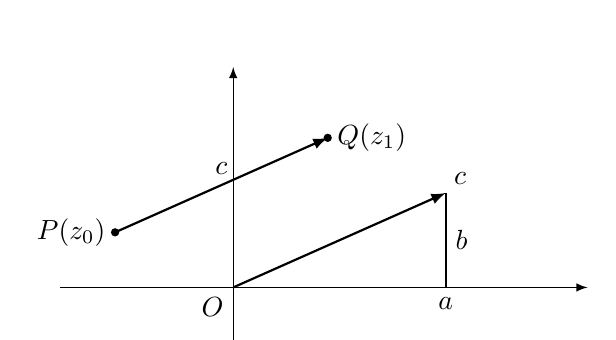
\begin{tikzpicture}[>=latex, scale=1.0]
  % Axes
  \draw[->] (-2.2, 0) -- (4.5, 0);
  \draw[->] (0, -0.8) -- (0, 2.8);
  \node[below left] at (0, 0) {$O$};
  
  % Left vector from P(z0) to Q(z1)
  \coordinate (P) at (-1.5, 0.7);
  \coordinate (Q) at (1.2, 1.9);
  \draw[->, thick] (P) -- (Q) node[midway, above] {$c$};
  \fill (P) circle (1.5pt) node[left] {$P(z_0)$};
  \fill (Q) circle (1.5pt) node[right] {$Q(z_1)$};
  
  % Right vector from O(0,0) to (a, b)
  \coordinate (C) at (2.7, 1.2);
  \draw[->, thick] (0, 0) -- (C) node[above right=-1pt] {$c$};
  \draw[thick] (2.7, 0) -- (C);
  \node[below] at (2.7, 0) {$a$};
  \node[right] at (2.7, 0.6) {$b$};
\end{tikzpicture}
\\[5pt]
\small 圖 2-1
\end{center}

所以當平面上向量 $\mathbf{c}$ 的複數座標 $c = z_1-z_0 = a+bi$ 時，它在原來的正交座標系的座標表示相應地就是 $(a, b)$．

以下我們更進一步列出平面上向量與複數之間的兩項密切關係：
\begin{itemize}
  \item[(i)] 設平面上向量 $\mathbf{c}_1, \mathbf{c}_2$ 的複數座標分別為 $c_1=a_1+b_1i$ 及 $c_2=a_2+b_2i$，則向量 $\mathbf{c}_1+\mathbf{c}_2$ 的複數座標是
  \[
  c_1+c_2 = (a_1+a_2)+(b_1+b_2)i.
  \]
  換句話說，\textbf{向量的加法對應於複數的加法}．
  \begin{center}
  \begin{minipage}{0.48\textwidth}
  \centering
  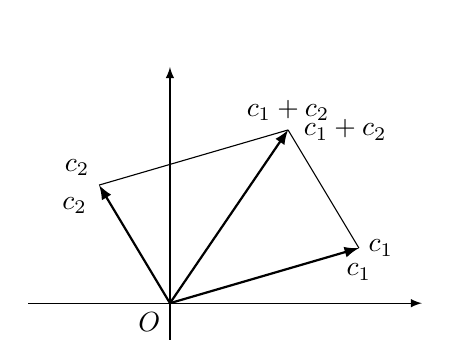
\begin{tikzpicture}[>=latex, scale=1.0]
    \draw[->] (-1.8, 0) -- (3.2, 0);
    \draw[->] (0, -0.6) -- (0, 3.0);
    \node[below left] at (0, 0) {$O$};
    
    \coordinate (C1) at (2.4, 0.7);
    \coordinate (C2) at (-0.9, 1.5);
    \coordinate (Sum) at (1.5, 2.2);
    
    \draw[->, thick] (0, 0) -- (C1) node[below=2pt] {$c_1$};
    \node[right] at (C1) {$c_1$};
    \draw[->, thick] (0, 0) -- (C2) node[below left=1pt] {$c_2$};
    \node[above left] at (C2) {$c_2$};
    \draw[->, thick] (0, 0) -- (Sum) node[right=2pt] {$c_1+c_2$};
    \node[above] at (Sum) {$c_1+c_2$};
    
    \draw (C1) -- (Sum);
    \draw (C2) -- (Sum);
  \end{tikzpicture}
  \\[5pt]
  \small 圖 2-2
  \end{minipage}
  \begin{minipage}{0.48\textwidth}
  \centering
  \begin{tikzpicture}[>=latex, scale=1.0]
    \draw[->] (-0.8, 0) -- (3.8, 0);
    \draw[->] (0, -0.6) -- (0, 2.8);
    \node[below left] at (0, 0) {$O$};
    
    \coordinate (C) at (1.6, 1.0);
    \coordinate (RC) at (3.0, 1.875);
    
    \draw[->, thick] (0, 0) -- (C) node[below right=1pt] {$c$};
    \draw[->, thick] (C) -- (RC) node[right=1pt] {$rc$};
    \node[below right] at (0.8, 0.5) {$c$};
    \node[below right] at (2.3, 1.44) {$rc$};
  \end{tikzpicture}
  \\[5pt]
  \small 圖 2-3
  \end{minipage}
  \end{center}

  \item[(ii)] 設平面上向量 $\mathbf{c}$ 的複數座標是 $c=a+bi$，並設 $r \in \mathbf{R}$ 是一個任意實數，則向量 $r\mathbf{c}$ 的複數座標是 $rc = ra+rbi$．換句話說，\textbf{向量的係數積對應於複數乘以實數}．
\end{itemize}

\begin{definition}[複數的絕對值]
當複數 $c=a+bi$ 是向量 $\mathbf{c}$ 的坐標時，我們定義複數 $c$ 的\textbf{絕對值} $|c|$ 等於向量 $\mathbf{c}$ 的長度 $|\mathbf{c}|$，亦即
\[
|c| = |\mathbf{c}| = \sqrt{a^2+b^2}.
\]
換句話說，複數的絕對值，對應於向量的長度．
\end{definition}

\begin{example-non}[例 2]
\[
|i| = \sqrt{0^2+1^2} = 1, \quad |1+i| = \sqrt{1^2+1^2} = \sqrt{2}.
\]
\end{example-non}

有了上面的定義，我們可以推出下面的公式：
\begin{align*}
|z_1+z_2| &\le |z_1|+|z_2|, \quad z_1, z_2 \in \mathbf{C}, \\
|z_1 z_2| &= |z_1||z_2|, \quad z_1, z_2 \in \mathbf{C}. \quad \text{證明留作習題.}
\end{align*}

\begin{example-non}[例 3]
設 $z$ 為複數，試求 $|z-2|+|z+2|=6$ 在複數平面上的圖形．
\end{example-non}

\begin{solution}
令 $P(x, y)$ 為圖形上點，其中 $z=x+yi$ 滿足 $|z-2|+|z+2|=6$．則由定義得
\[
\sqrt{(x-2)^2+y^2} + \sqrt{(x+2)^2+y^2} = 6.
\]
上式表示：點 $P(x, y)$ 至二定點 $F(2, 0)$ 及 $F'(-2, 0)$ 的距離和恆為 $6$，故圖形為一橢圓．（若把 $z-2$ 看成向量 $\overrightarrow{PF}$，$|z-2|$ 為 $|\overrightarrow{PF}|$，則結論相同且更為直捷，這是複數表示簡單明瞭的優點）． \qedhere
\end{solution}

\subsubsection*{作業 4}
設 $z$ 為複數，試求下列方程式在複數平面上的圖形：
\begin{itemize}
  \item[(i)] $|z-i|-|z+i|=5$
  \item[(ii)] $|z-1+2i|=3$
\end{itemize}


\subsubsection*{丙、複數乘法與複角公式}

設 $C$ 為以原點為圓心，半徑為 $1$ 的單位圓，並設 $P_1, P_2$ 是 $C$ 上任給兩點，如下圖所示，其複數座標分別為 $z_1, z_2$．若 $\theta_1, \theta_2$ 分別為 $\overrightarrow{OP_1}, \overrightarrow{OP_2}$ 和 $x$-軸的夾角，則得
\[
\overrightarrow{OP_1} = (\cos\theta_1, \sin\theta_1), \quad \overrightarrow{OP_2} = (\cos\theta_2, \sin\theta_2),
\]
亦即
\[
z_1 = \cos\theta_1+i\sin\theta_1, \quad z_2 = \cos\theta_2+i\sin\theta_2.
\]

\begin{center}
\begin{minipage}{0.48\textwidth}
由複數的乘法公式得
\begin{align*}
z_1 z_2 &= (\cos\theta_1+i\sin\theta_1)(\cos\theta_2+i\sin\theta_2) \\
&= (\cos\theta_1\cos\theta_2 - \sin\theta_1\sin\theta_2) \\
&\quad + i(\cos\theta_1\sin\theta_2 + \cos\theta_2\sin\theta_1).
\end{align*}
另一方面，由餘弦與正弦的複角公式，即有
\[
z_1 z_2 = \cos(\theta_1+\theta_2)+i\sin(\theta_1+\theta_2).
\]
\end{minipage}
\hfill
\begin{minipage}{0.48\textwidth}
\centering
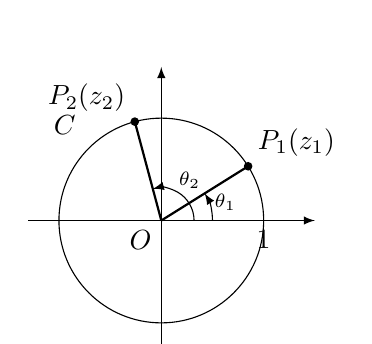
\begin{tikzpicture}[>=latex, scale=1.3]
  \draw[->] (-1.3,0) -- (1.5,0);
  \draw[->] (0,-1.3) -- (0,1.5);
  \draw (0,0) circle (1.0);
  \node[below left] at (0,0) {$O$};
  \node[below] at (1,0) {$1$};
  \node[above left] at (135:1.05) {$C$};
  
  \coordinate (P1) at (32:1.0);
  \coordinate (P2) at (105:1.0);
  
  \draw[thick] (0,0) -- (P1);
  \fill (P1) circle (1.2pt) node[above right] {$P_1(z_1)$};
  
  \draw[thick] (0,0) -- (P2);
  \fill (P2) circle (1.2pt) node[above left] {$P_2(z_2)$};
  
  \draw[->] (0.5,0) arc (0:32:0.5);
  \node at (16:0.65) {\scriptsize $\theta_1$};
  
  \draw[->] (0.32,0) arc (0:105:0.32);
  \node at (55:0.48) {\scriptsize $\theta_2$};
\end{tikzpicture}
\\[5pt]
\small 圖 2-4
\end{minipage}
\end{center}

因此我們得到
\[
(\cos\theta_1+i\sin\theta_1)(\cos\theta_2+i\sin\theta_2) = \cos(\theta_1+\theta_2)+i\sin(\theta_1+\theta_2).
\]
上述公式的意義有二：一方面它利用複數乘法把三角函數的複角公式改寫成上述簡單易記的形式，我們只要把上式左端展開，即得到原來的兩個複角公式：
\begin{align*}
\cos(\theta_1+\theta_2) &= \cos\theta_1\cos\theta_2 - \sin\theta_1\sin\theta_2, \\
\sin(\theta_1+\theta_2) &= \cos\theta_1\sin\theta_2 + \cos\theta_2\sin\theta_1.
\end{align*}

另一方面它顯示了複數乘法所對應的幾何意義：

\begin{center}
\begin{minipage}{0.52\textwidth}
對於任給兩個複數 $z_1, z_2 \in \mathbf{C}$，
\begin{align*}
z_1 &= |z_1|(\cos\theta_1+i\sin\theta_1), \\
z_2 &= |z_2|(\cos\theta_2+i\sin\theta_2)
\end{align*}
（稱為複數的\textbf{極式}，詳見 § V-3，甲）

其中 $\theta_1, \theta_2$ 分別叫做 $z_1, z_2$ 的\textbf{幅角}．

〔註〕如圖所示，記作 $\theta_1 = \arg z_1$，$\theta_2 = \arg z_2$（$\arg$ 為 argument 之簡寫）．
\end{minipage}
\hfill
\begin{minipage}{0.45\textwidth}
\centering
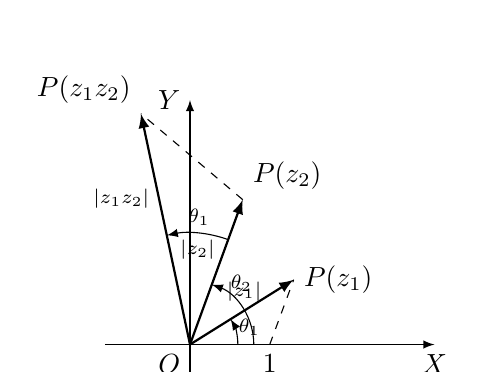
\begin{tikzpicture}[>=latex, scale=1.35]
  \draw[->] (-0.8,0) -- (2.3,0) node[below] {$X$};
  \draw[->] (0,-0.3) -- (0,2.3) node[left] {$Y$};
  \node[below left] at (0,0) {$O$};
  
  \coordinate (U) at (0.75,0);
  \node[below] at (U) {$1$};
  
  \coordinate (P1) at (32:1.15);
  \coordinate (P2) at (70:1.45);
  \coordinate (P12) at (102:2.22);
  
  % Vectors
  \draw[->, thick] (0,0) -- (P1) node[right] {$P(z_1)$};
  \draw[->, thick] (0,0) -- (P2) node[above right] {$P(z_2)$};
  \draw[->, thick] (0,0) -- (P12) node[above left] {$P(z_1 z_2)$};
  
  % Similar triangles dashed lines
  \draw[dashed] (U) -- (P1);
  \draw[dashed] (P2) -- (P12);
  
  % Length labels
  \node[above] at (32:0.6) {\scriptsize $|z_1|$};
  \node[left] at (70:0.95) {\scriptsize $|z_2|$};
  \node[left] at (102:1.4) {\scriptsize $|z_1 z_2|$};
  
  % Angle arcs
  \draw[->] (0.45,0) arc (0:32:0.45);
  \node at (16:0.58) {\scriptsize $\theta_1$};
  
  \draw[->] (0.6,0) arc (0:70:0.6);
  \node at (50:0.75) {\scriptsize $\theta_2$};
  
  \draw[->] (70:1.05) arc (70:102:1.05);
  \node at (86:1.2) {\scriptsize $\theta_1$};
\end{tikzpicture}
\\[5pt]
\small 圖 2-5
\end{minipage}
\end{center}

由上述公式即得
\begin{align*}
z_1 z_2 &= |z_1|(\cos\theta_1+i\sin\theta_1)\cdot |z_2|(\cos\theta_2+i\sin\theta_2) \\
&= |z_1||z_2|(\cos\theta_1+i\sin\theta_1)(\cos\theta_2+i\sin\theta_2) \\
&= |z_1||z_2|[\cos(\theta_1+\theta_2)+i\sin(\theta_1+\theta_2)].
\end{align*}
換句話說，\textbf{當兩個複數相乘時，其絕對值相乘而其幅角相加}．

\begin{footnote}
幅角本身多值，彼此之間相差 $2\pi$ 的整數倍，取其中介於 $-\pi$ 與 $\pi$ 間的那一個，作為\textbf{主幅角}．
\end{footnote}

\subsubsection*{作業 5}
\begin{itemize}
  \item[(i)] 試用歸納法證明棣美佛（De Moivre）公式：
  \[
  (\cos\theta+i\sin\theta)^n = \cos n\theta+i\sin n\theta, \quad n \in \mathbf{N}.
  \]
  〔事實上此公式中的 $n$ 可推廣至所有實數，這在 § V-3 甲段引入複數的指數形式後從指數定則就很容看出．〕
  \item[(ii)] 若 $z=|z|(\cos\theta+i\sin\theta)$，證明並圖解
  \[
  \frac{1}{z} = \frac{1}{|z|}(\cos\theta-i\sin\theta).
  \]
  \item[(iii)] 若 $z_1=|z_1|(\cos\theta_1+i\sin\theta_1), z_2=|z_2|(\cos\theta_2+i\sin\theta_2)$，證明並圖解
  \[
  \frac{z_1}{z_2} = \frac{|z_1|}{|z_2|}[\cos(\theta_1-\theta_2)+i\sin(\theta_1-\theta_2)].
  \]
\end{itemize}


\begin{example-non}[例 4]
設 $\alpha = \rho(\cos\theta+i\sin\theta), \beta = r(\cos\phi+i\sin\phi)$，試求 $\dfrac{\alpha+\beta}{\alpha-\beta}$ 之實部．
\end{example-non}

\begin{solution}
\begin{align*}
\alpha+\beta &= (\rho\cos\theta+r\cos\phi)+i(\rho\sin\theta+r\sin\phi), \\
\alpha-\beta &= (\rho\cos\theta-r\cos\phi)+i(\rho\sin\theta-r\sin\phi).
\end{align*}
而 $\dfrac{a+bi}{c+di} = \dfrac{ac+bd}{c^2+d^2} + \dfrac{bc-ad}{c^2+d^2}i$，故經代入求簡化後可得所求 $\dfrac{\alpha+\beta}{\alpha-\beta}$ 之實部為
\[
\frac{\rho^2-r^2}{\rho^2+r^2-2\rho r\cos(\theta-\phi)}. \qedhere
\]
\end{solution}

\begin{example-non}[例 5]
試圖示下列各複數，並表為極式：
\begin{itemize}
  \item[(i)] $3+3i$
  \item[(ii)] $-1+\sqrt{3}i$
  \item[(iii)] $-1$
  \item[(iv)] $-2-2\sqrt{3}i$
\end{itemize}
\end{example-non}

\begin{solution}
\begin{center}
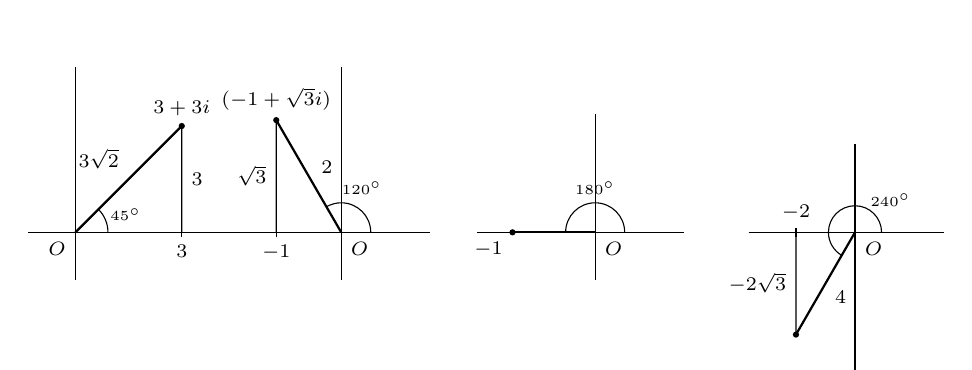
\begin{tikzpicture}[>=latex, scale=0.75]
  % (i) 3+3i
  \begin{scope}[shift={(0,0)}]
    \draw (-0.8,0) -- (2.8,0);
    \draw (0,-0.8) -- (0,2.8);
    \coordinate (P) at (1.8,1.8);
    \draw[thick] (0,0) -- (P);
    \fill (P) circle (1.5pt) node[above] {\scriptsize $3+3i$};
    \draw (1.8,0) -- (P);
    \draw (0.55,0) arc (0:45:0.55);
    \node at (0.85,0.3) {\tiny $45^\circ$};
    \draw (1.8,-0.08) -- (1.8,0.08);
    \node[below] at (1.8,-0.05) {\scriptsize $3$};
    \node[right] at (1.8,0.9) {\scriptsize $3$};
    \node[above left] at (0.9,0.9) {\scriptsize $3\sqrt{2}$};
    \node[below left] at (0,0) {\scriptsize $O$};
  \end{scope}

  % (ii) -1 + sqrt(3)i
  \begin{scope}[shift={(4.5,0)}]
    \draw (-1.8,0) -- (1.5,0);
    \draw (0,-0.8) -- (0,2.8);
    \coordinate (P) at (-1.1,1.9);
    \draw[thick] (0,0) -- (P);
    \fill (P) circle (1.5pt) node[above] {\scriptsize $(-1+\sqrt{3}i)$};
    \draw (-1.1,0) -- (P);
    \draw (0.5,0) arc (0:120:0.5);
    \node at (0.35,0.75) {\tiny $120^\circ$};
    \draw (-1.1,-0.08) -- (-1.1,0.08);
    \node[below] at (-1.1,-0.05) {\scriptsize $-1$};
    \node[left] at (-1.1,0.95) {\scriptsize $\sqrt{3}$};
    \node[right] at (-0.5,1.1) {\scriptsize $2$};
    \node[below right] at (0,0) {\scriptsize $O$};
  \end{scope}

  % (iii) -1
  \begin{scope}[shift={(8.8,0)}]
    \draw (-2.0,0) -- (1.5,0);
    \draw (0,-0.8) -- (0,2.0);
    \draw[thick] (0,0) -- (-1.4,0);
    \fill (-1.4,0) circle (1.5pt);
    \draw (0.5,0) arc (0:180:0.5);
    \node at (0,0.75) {\tiny $180^\circ$};
    \node[below left] at (-1.4,0) {\scriptsize $-1$};
    \node[below right] at (0,0) {\scriptsize $O$};
  \end{scope}

  % (iv) -2 - 2sqrt(3)i
  \begin{scope}[shift={(13.2,0)}]
    \draw (-1.8,0) -- (1.5,0);
    \draw (0,-2.5) -- (0,1.5);
    \coordinate (P) at (-1.0,-1.732);
    \draw[thick] (0,0) -- (P);
    \fill (P) circle (1.5pt);
    \draw (-1.0,0) -- (P);
    \draw (0.45,0) arc (0:240:0.45);
    \node at (0.6,0.55) {\tiny $240^\circ$};
    \draw (-1.0,-0.08) -- (-1.0,0.08);
    \node[above] at (-1.0,0.05) {\scriptsize $-2$};
    \node[left] at (-1.0,-0.86) {\scriptsize $-2\sqrt{3}$};
    \node[right] at (-0.5,-1.1) {\scriptsize $4$};
    \node[below right] at (0,0) {\scriptsize $O$};
  \end{scope}
\end{tikzpicture}
\\[5pt]
\small 圖 2-6
\end{center}

\begin{itemize}
  \item[(i)] 幅角 $\theta = \dfrac{\pi}{4}$，$|3+3i| = \sqrt{3^2+3^2} = 3\sqrt{2}$． \\
  $\therefore 3+3i = |3+3i|\left(\cos\dfrac{\pi}{4}+i\sin\dfrac{\pi}{4}\right)$．
  \item[(ii)] 幅角 $\theta = \dfrac{2\pi}{3}$，$|-1+\sqrt{3}i| = \sqrt{(-1)^2+(\sqrt{3})^2} = 2$． \\
  $\therefore -1+\sqrt{3}i = 2\left(\cos\dfrac{2\pi}{3}+i\sin\dfrac{2\pi}{3}\right)$．
  \item[(iii)] 幅角 $\theta = \pi$，$|-1| = \sqrt{(-1)^2+0^2} = 1$． \\
  $\therefore -1 = 1\cdot(\cos\pi+i\sin\pi) = \cos\pi+i\sin\pi$．
  \item[(iv)] 幅角 $\theta = \dfrac{4\pi}{3}$，$|-2-2\sqrt{3}i| = \sqrt{(-2)^2+(-2\sqrt{3})^2} = 4$． \\
  $\therefore -2-2\sqrt{3}i = 4\left(\cos\dfrac{4\pi}{3}+i\sin\dfrac{4\pi}{3}\right)$． \qedhere
\end{itemize}
\end{solution}

\begin{example-non}[例 6]
求 $(-1+\sqrt{3}i)^{10}$．
\end{example-non}

\begin{solution}
$\because -1+\sqrt{3}i = 2\left(\cos\dfrac{2\pi}{3}+i\sin\dfrac{2\pi}{3}\right)$． \\
$\therefore$ 由棣美佛定理得
\begin{align*}
(-1+\sqrt{3}i)^{10} &= \left[2\left(\cos\frac{2\pi}{3}+i\sin\frac{2\pi}{3}\right)\right]^{10} \\
&= 2^{10}\left(\cos\frac{20\pi}{3}+i\sin\frac{20\pi}{3}\right) \\
&= 1024\left[\cos\left(6\pi+\frac{2\pi}{3}\right)+i\sin\left(6\pi+\frac{2\pi}{3}\right)\right] \\
&= 1024\left(\cos\frac{2\pi}{3}+i\sin\frac{2\pi}{3}\right) \\
&= 1024\left(-\frac{1}{2}+\frac{\sqrt{3}}{2}i\right) \\
&= -512+512\sqrt{3}i. \qedhere
\end{align*}
\end{solution}

\subsubsection*{作業 6}
\begin{itemize}
  \item[(i)] 試求 $(1+i)^n + (1-i)^n$．
  \item[(ii)] 圖示各複數 $1+i, 1-2i, \sqrt{3}-i$，並表為極式．
  \item[(iii)] 設 $\alpha = 1+i, \beta = 1-2i$，試求 $\dfrac{\alpha-\beta}{\alpha+\beta}$ 之實部．
\end{itemize}


\subsubsection*{丁、$n$ 次方根}

我們考慮 $z^n-c=0, c \neq 0, (n \in \mathbf{N})$．這個方程式的解叫做複數 $c$ 的 \textbf{$n$ 次方根}或簡稱\textbf{方根}．當 $n=2, 3$ 時，$n$ 方根常分別稱為平方根，立方根．在 § V-1 的論例 1 中我們討論過平方根這個最簡單的情形，但是所用的解法對於高次的情形是不適用的．譬如當 $n=5$ 時，
\begin{align*}
(x+yi)^5-(a+bi) &= (x^5-10x^3 y^2+5xy^4-a) \\
&\quad + (5x^4 y-10x^2 y^3+y^5-b)i = 0,
\end{align*}
用同樣的解法則需要解聯立方程式：
\[
\begin{cases}
x^5-10x^3 y^2+5xy^4-a = 0, \\
5x^4 y-10x^2 y^3+y^5-b = 0.
\end{cases}
\]
這是一個很複雜難解的二元高次方程組．但若我們利用丙段所得的結果——複數乘法的幾何意義，則一般 $n$ 次方根就可以直截了當地解出：

設 $z$ 的幅角為 $\theta$，$c$ 的幅角為 $\gamma$（$\arg z = \theta, \arg c = \gamma$），則
\[
z = |z|(\cos\theta+i\sin\theta), \quad c = |c|(\cos\gamma+i\sin\gamma).
\]
而 $z$ 滿足方程式 $z^n-c=0$，故有
\begin{align*}
z^n-c &= \{|z|(\cos\theta+i\sin\theta)\}^n - |c|(\cos\gamma+i\sin\gamma) \\
&= |z|^n(\cos\theta+i\sin\theta)^n - |c|(\cos\gamma+i\sin\gamma) \\
&= |z|^n(\cos n\theta+i\sin n\theta) - |c|(\cos\gamma+i\sin\gamma) = 0.
\end{align*}
由於 $|z|^n = |c|$ 得 $|z| = \sqrt[n]{|c|}$．因此由上式我們得到
\[
\cos n\theta = \cos\gamma, \quad \sin n\theta = \sin\gamma.
\]
由正弦與餘弦函數的週期性，可知：
\[
n\theta = 2k\pi+\gamma, \quad k \in \mathbf{Z},
\]
即
\[
\theta = \frac{\gamma+2k\pi}{n}, \quad k \in \mathbf{Z},
\]
所以方程式 $z^n-c=0$ 的解可以寫成下列形式
\[
z = \sqrt[n]{|c|}\left(\cos\frac{\gamma+2k\pi}{n} + i\sin\frac{\gamma+2k\pi}{n}\right), \quad k \in \mathbf{Z}.
\]
再由 $\cos, \sin$ 的週期性（週期為 $2\pi$）不難看出上式中共有 $n$ 個不同的值，即
\[
z_k = \sqrt[n]{|c|}\left(\cos\frac{\gamma+2k\pi}{n} + i\sin\frac{\gamma+2k\pi}{n}\right), \quad k=0, 1, 2, \dots, n-1.
\]
這 $n$ 個值也就是複數 $c=|c|(\cos\gamma+i\sin\gamma)$ 的 $n$ 個不同的方根．

當 $c$ 為正實數時，仍用 $\sqrt[n]{c}$ 表示其中的正實根；當 $c$ 不是正實數時，則用 $\sqrt[n]{c}$ 表示其中的任一個．

\begin{example-non}[論例 3]
當 $c=1$ 時，$|c|=1$，幅角 $\arg c = 0$，故 $z^n-1=0$ 的 $n$ 個解為
\begin{align*}
z_0 &= 1, \\
z_1 &= \cos\frac{2\pi}{n}+i\sin\frac{2\pi}{n}, \\
&\dots\dots\dots\dots\dots \\
z_{n-1} &= \cos\frac{2(n-1)\pi}{n}+i\sin\frac{2(n-1)\pi}{n}.
\end{align*}
由棣美佛定理不難看出 $z_2 = z_1^2, z_3 = z_1^3, \dots, z_{n-1} = z_1^{n-1}$．若令
\[
\omega_n = z_1 = \cos\frac{2\pi}{n}+i\sin\frac{2\pi}{n},
\]
則 $1$ 的 $n$ 個方根就是：$1, \omega_n, \omega_n^2, \dots, \omega_n^{n-1}$． \qedhere
\end{example-non}

\paragraph{推論} 利用上例中的 $1$ 的 $n$ 方根 $\omega_n$，則任意複數 $c=|c|(\cos\gamma+i\sin\gamma)$ 的 $n$ 方根可寫為
\[
z_0 = \sqrt[n]{|c|}\left(\cos\frac{\gamma}{n}+i\sin\frac{\gamma}{n}\right), \quad z_1 = z_0\omega_n, \dots, z_{n-1} = z_0\omega_n^{n-1}.
\]

茲以簡單的例子，把上面討論的結果圖示如下：

\begin{center}
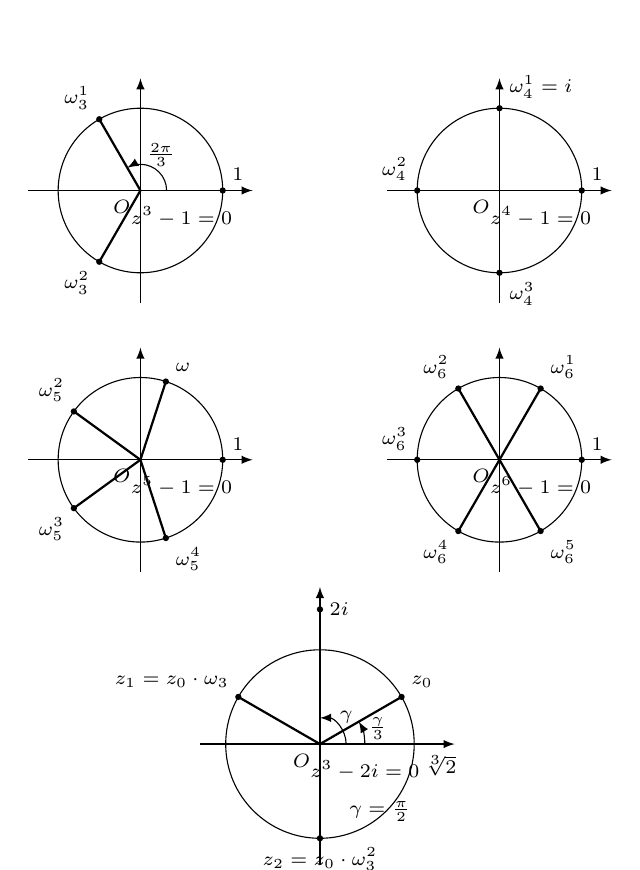
\begin{tikzpicture}[>=latex, scale=0.95]
  % (1) z^3-1=0
  \begin{scope}[shift={(0,3.6)}]
    \draw[->] (-1.5,0) -- (1.5,0);
    \draw[->] (0,-1.5) -- (0,1.5);
    \draw (0,0) circle (1.1);
    \node[below left] at (0,0) {\scriptsize $O$};
    \node at (0.55,-0.35) {\scriptsize $z^3-1=0$};
    
    \coordinate (A0) at (0:1.1);
    \coordinate (A1) at (120:1.1);
    \coordinate (A2) at (240:1.1);
    
    \fill (A0) circle (1.2pt) node[above right] {\scriptsize $1$};
    \draw[thick] (0,0) -- (A1);
    \fill (A1) circle (1.2pt) node[above left] {\scriptsize $\omega_3^1$};
    \draw[thick] (0,0) -- (A2);
    \fill (A2) circle (1.2pt) node[below left] {\scriptsize $\omega_3^2$};
    
    \draw[->] (0.35,0) arc (0:120:0.35);
    \node at (60:0.55) {\scriptsize $\frac{2\pi}{3}$};
  \end{scope}

  % (2) z^4-1=0
  \begin{scope}[shift={(4.8,3.6)}]
    \draw[->] (-1.5,0) -- (1.5,0);
    \draw[->] (0,-1.5) -- (0,1.5);
    \draw (0,0) circle (1.1);
    \node[below left] at (0,0) {\scriptsize $O$};
    \node at (0.55,-0.35) {\scriptsize $z^4-1=0$};
    
    \coordinate (B0) at (0:1.1);
    \coordinate (B1) at (90:1.1);
    \coordinate (B2) at (180:1.1);
    \coordinate (B3) at (270:1.1);
    
    \fill (B0) circle (1.2pt) node[above right] {\scriptsize $1$};
    \fill (B1) circle (1.2pt) node[above right] {\scriptsize $\omega_4^1=i$};
    \fill (B2) circle (1.2pt) node[above left] {\scriptsize $\omega_4^2$};
    \fill (B3) circle (1.2pt) node[below right] {\scriptsize $\omega_4^3$};
  \end{scope}

  % (3) z^5-1=0
  \begin{scope}[shift={(0,0)}]
    \draw[->] (-1.5,0) -- (1.5,0);
    \draw[->] (0,-1.5) -- (0,1.5);
    \draw (0,0) circle (1.1);
    \node[below left] at (0,0) {\scriptsize $O$};
    \node at (0.55,-0.35) {\scriptsize $z^5-1=0$};
    
    \fill (0:1.1) circle (1.2pt) node[above right] {\scriptsize $1$};
    \draw[thick] (0,0) -- (72:1.1);
    \fill (72:1.1) circle (1.2pt) node[above right] {\scriptsize $\omega$};
    \draw[thick] (0,0) -- (144:1.1);
    \fill (144:1.1) circle (1.2pt) node[above left] {\scriptsize $\omega_5^2$};
    \draw[thick] (0,0) -- (216:1.1);
    \fill (216:1.1) circle (1.2pt) node[below left] {\scriptsize $\omega_5^3$};
    \draw[thick] (0,0) -- (288:1.1);
    \fill (288:1.1) circle (1.2pt) node[below right] {\scriptsize $\omega_5^4$};
  \end{scope}

  % (4) z^6-1=0
  \begin{scope}[shift={(4.8,0)}]
    \draw[->] (-1.5,0) -- (1.5,0);
    \draw[->] (0,-1.5) -- (0,1.5);
    \draw (0,0) circle (1.1);
    \node[below left] at (0,0) {\scriptsize $O$};
    \node at (0.55,-0.35) {\scriptsize $z^6-1=0$};
    
    \fill (0:1.1) circle (1.2pt) node[above right] {\scriptsize $1$};
    \draw[thick] (0,0) -- (60:1.1);
    \fill (60:1.1) circle (1.2pt) node[above right] {\scriptsize $\omega_6^1$};
    \draw[thick] (0,0) -- (120:1.1);
    \fill (120:1.1) circle (1.2pt) node[above left] {\scriptsize $\omega_6^2$};
    \fill (180:1.1) circle (1.2pt) node[above left] {\scriptsize $\omega_6^3$};
    \draw[thick] (0,0) -- (240:1.1);
    \fill (240:1.1) circle (1.2pt) node[below left] {\scriptsize $\omega_6^4$};
    \draw[thick] (0,0) -- (300:1.1);
    \fill (300:1.1) circle (1.2pt) node[below right] {\scriptsize $\omega_6^5$};
  \end{scope}

  % (5) z^3-2i=0
  \begin{scope}[shift={(2.4,-3.8)}]
    \draw[->] (-1.6,0) -- (1.8,0);
    \draw[->] (0,-1.6) -- (0,2.1);
    \draw (0,0) circle (1.26);
    \node[below left] at (0,0) {\scriptsize $O$};
    \node at (0.6,-0.35) {\scriptsize $z^3-2i=0$};
    \node[below right] at (1.26,-0.02) {\scriptsize $\sqrt[3]{2}$};
    
    \fill (0,1.8) circle (1.2pt) node[right] {\scriptsize $2i$};
    
    \coordinate (C0) at (30:1.26);
    \coordinate (C1) at (150:1.26);
    \coordinate (C2) at (270:1.26);
    
    \draw[thick] (0,0) -- (C0);
    \fill (C0) circle (1.2pt) node[above right] {\scriptsize $z_0$};
    
    \draw[thick] (0,0) -- (C1);
    \fill (C1) circle (1.2pt) node[above left] {\scriptsize $z_1=z_0\cdot\omega_3$};
    
    \fill (C2) circle (1.2pt) node[below] {\scriptsize $z_2=z_0\cdot\omega_3^2$};
    
    \draw[->] (0.6,0) arc (0:30:0.6);
    \node at (15:0.8) {\scriptsize $\frac{\gamma}{3}$};
    
    \draw[->] (0.35,0) arc (0:90:0.35);
    \node at (45:0.5) {\scriptsize $\gamma$};
    
    \node at (0.8,-0.9) {\scriptsize $\gamma=\frac{\pi}{2}$};
  \end{scope}
\end{tikzpicture}
\\[5pt]
\small 圖 2-7
\end{center}

\begin{example-non}[論例 4]
設 $P_1(z_1), P_2(z_2), P_3(z_3)$ 及 $P_4(z_4)$ 是複數平面上互不共線的四點．試求其共圓的充分及必要條件．
\end{example-non}

\begin{solution}
\begin{center}
\begin{minipage}{0.55\textwidth}
向量 $\overrightarrow{P_2 P_1}$ 的複數坐標為 $z_1-z_2$，\\
$\overrightarrow{P_2 P_3}$ 的複數坐標為 $z_3-z_2$，\\
$\overrightarrow{P_4 P_1}$ 的複數坐標為 $z_1-z_4$，\\
$\overrightarrow{P_4 P_3}$ 的複數坐標為 $z_3-z_4$．

由複數乘法的幾何意義即得
\begin{align*}
\arg\frac{z_1-z_2}{z_3-z_2} &= \overrightarrow{P_2 P_1}\text{ 的幅角} - \overrightarrow{P_2 P_3}\text{ 的幅角} = \theta_2, \\
\arg\frac{z_3-z_4}{z_1-z_4} &= \overrightarrow{P_4 P_3}\text{ 的幅角} - \overrightarrow{P_4 P_1}\text{ 的幅角} = \theta_4.
\end{align*}
\end{minipage}
\hfill
\begin{minipage}{0.42\textwidth}
\centering
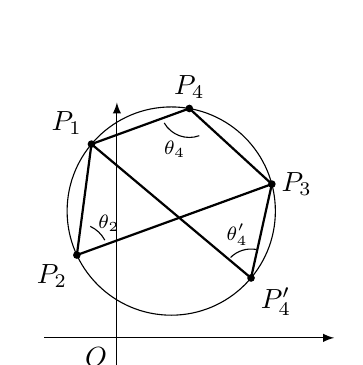
\begin{tikzpicture}[>=latex, scale=1.15]
  \draw[->] (-0.8,0) -- (2.4,0);
  \draw[->] (0,-0.4) -- (0,2.6);
  \node[below left] at (0,0) {$O$};
  
  \coordinate (Center) at (0.6,1.4);
  \draw (Center) circle (1.15);
  
  \coordinate (P1) at ($(Center)+(140:1.15)$);
  \coordinate (P2) at ($(Center)+(205:1.15)$);
  \coordinate (P3) at ($(Center)+(15:1.15)$);
  \coordinate (P4) at ($(Center)+(80:1.15)$);
  \coordinate (P4p) at ($(Center)+(320:1.15)$);
  
  \draw[thick] (P1) -- (P2) -- (P3);
  \draw[thick] (P1) -- (P4) -- (P3);
  \draw[thick] (P1) -- (P4p) -- (P3);
  
  \fill (P1) circle (1.2pt) node[above left] {$P_1$};
  \fill (P2) circle (1.2pt) node[below left] {$P_2$};
  \fill (P3) circle (1.2pt) node[right] {$P_3$};
  \fill (P4) circle (1.2pt) node[above] {$P_4$};
  \fill (P4p) circle (1.2pt) node[below right] {$P_4'$};
  
  \draw ($(P2)+(28:0.35)$) arc (28:65:0.35);
  \node at ($(P2)+(45:0.5)$) {\scriptsize $\theta_2$};
  
  \draw ($(P4)+(210:0.32)$) arc (210:290:0.32);
  \node at ($(P4)+(250:0.48)$) {\scriptsize $\theta_4$};
  
  \draw ($(P4p)+(80:0.32)$) arc (80:135:0.32);
  \node at ($(P4p)+(108:0.5)$) {\scriptsize $\theta_4'$};
\end{tikzpicture}
\\[5pt]
\small 圖 2-8
\end{minipage}
\end{center}

因而互不共線四點 $P_1, P_2, P_3, P_4$ 共圓的充分及必要條件為
\[
\theta_2+\theta_4 = \pm\pi \quad \text{（如圖中 $P_1 P_2 P_3 P_4$ 的情形），}
\]
或
\[
\theta_2+\theta_4' = 0 \quad \text{（如圖中 $P_1 P_2 P_3 P_4'$ 的情形）.}
\]
把這個條件改用複數表示即為
\[
\arg\left(\frac{z_1-z_2}{z_3-z_2}\cdot\frac{z_3-z_4}{z_1-z_4}\right) = \pm\pi \text{ 或 } 0.
\]
但是一個複數的幅角等於 $0$ 時，則它是一個正實數，而幅角等於 $\pm\pi$ 時，則它是一個負實數．因此互不共線的四點 $P_1, P_2, P_3, P_4$ 共圓的條件是其複數坐標滿足下列條件：
\begin{equation}
\frac{z_1-z_2}{z_3-z_2}\cdot\frac{z_3-z_4}{z_1-z_4} = t \in \mathbf{R}. \tag{A}
\end{equation}
如果 $P_1, P_2, P_3, P_4$ 四點共線，上述條件 (A) 顯然成立．綜合這兩種情形，我們得到下列結果：
\[
P_1, P_2, P_3, P_4 \text{ 四點共圓或共線} \iff \text{條件 (A) 成立.} \qedhere
\]
\end{solution}

\begin{example-non}[論例 5]
設 $P_1, P_2, P_3$ 是平面上任給不共線之點，其複數坐標分別為 $z_1, z_2, z_3$．令 $\Gamma$ 為 $P_1, P_2, P_3$ 三點所決定的圓．若 $P(z) \in \Gamma$ 是圓上任意一點，則由上例可知
\[
\frac{z_1-z_2}{z_3-z_2}\cdot\frac{z_3-z}{z_1-z} = t \in \mathbf{R}.
\]
由上式解出 $z$：
\[
z = \frac{(z_3-z_2)z_1 t + (z_2-z_1)z_3}{(z_3-z_2)t + (z_2-z_1)}, \quad t \in \mathbf{R}.
\]
換句話說，利用一個實數參數 $t \in \mathbf{R}$，我們可以把圓 $\Gamma$ 上的任意一點 $P(z)$ 的複數坐標用上式表示，所以上式也就是由 $P_1(z_1), P_2(z_2), P_3(z_3)$ 三點所決定的圓 $\Gamma$ 的複數坐標的參數方程式．我們可以看出：
\begin{align*}
t=0 \text{ 時，} \quad & z = z_3, \\
t=1 \text{ 時，} \quad & z = z_2,
\end{align*}
當 $t$ 自 $-\infty$ 變至 $+\infty$ 時，則 $P(z)$ 由 $P_1$ 的一側繞圓一周到 $P_1$ 的另一側．
\end{example-non}

\subsubsection*{作業 7}
\begin{itemize}
  \item[(i)] 試討論 $P_1, P_2, P_3$ 三點共線時的情形．
  \item[(ii)] 設 $P_1, P_2$ 兩點決定一直線，試求其參數方程式．
\end{itemize}


\subsubsection*{戊、共軛與$^*$鏡射}

現在我們來考慮平面上的點對於 $X$-軸的鏡射（反射或反映）．設 $P(z)$ 是平面上任意一點，其複數座標為 $z=x+yi$，則 $P$ 對於 $X$-軸鏡射的像點，也就是關於 $X$-軸的對稱點 $\bar{P}$ 的座標為 $x-yi$．

\begin{center}
\begin{minipage}{0.55\textwidth}
\begin{definition}
設複數 $z=x+yi$，則複數 $\bar{z}=x-yi$ 叫做 $z$ 的\textbf{共軛複數}．
\end{definition}
由於 $\bar{\bar{z}} = x+yi = z$，所以 $z$ 也是 $\bar{z}$ 的共軛複數．我們也說 $z$ 與 $\bar{z}$ 互為共軛．
\end{minipage}
\hfill
\begin{minipage}{0.42\textwidth}
\centering
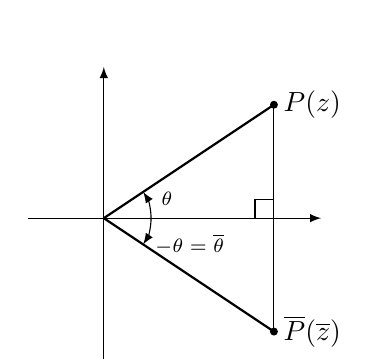
\begin{tikzpicture}[>=latex, scale=1.2]
  \draw[->] (-0.8,0) -- (2.3,0);
  \draw[->] (0,-1.6) -- (0,1.6);
  
  \coordinate (P) at (1.8,1.2);
  \coordinate (Pbar) at (1.8,-1.2);
  
  \draw[thick] (0,0) -- (P);
  \fill (P) circle (1.2pt) node[right] {$P(z)$};
  
  \draw[thick] (0,0) -- (Pbar);
  \fill (Pbar) circle (1.2pt) node[right] {$\bar{P}(\bar{z})$};
  
  \draw (P) -- (Pbar);
  \draw (1.8,0.2) -- (1.6,0.2) -- (1.6,0);
  
  \draw[->] (0.5,0) arc (0:33.7:0.5);
  \node at (17:0.7) {\scriptsize $\theta$};
  
  \draw[->] (0.5,0) arc (0:-33.7:0.5);
  \node at (-17:0.95) {\scriptsize $-\theta=\bar{\theta}$};
\end{tikzpicture}
\\[5pt]
\small 圖 2-9
\end{minipage}
\end{center}

由共軛的定義，我們有下列重要的結果：

設 $z=x+yi, \bar{z}=x-yi$ 為共軛複數，則
\begin{enumerate}
  \item $|z| = |\bar{z}| = \sqrt{x^2+y^2}$,
  \item $|z|^2 = |\bar{z}|^2 = x^2+y^2 = z\bar{z}$,
  \item $\arg z + \arg\bar{z} = \theta+\bar{\theta} = 0, \quad \bar{\theta} = -\theta$,
  \item $z+\bar{z} = 2x \in \mathbf{R}$ （共軛複數相加得實數），\\
  $z-\bar{z} = 2yi$ （共軛複數相減得虛數），
  \item $z = \bar{z} \iff z \in \mathbf{R}$，\\
  $z = -\bar{z} \iff z$ 為純虛數．
\end{enumerate}

\begin{example-non}[例 7]
\begin{itemize}
  \item[(i)] $\bar{i} = -i, \quad \overline{-i} = i$．
  \item[(ii)] 若 $z=\cos\theta+i\sin\theta$，亦即 $|z|=1$，則由 (2) $z\bar{z}=|z|^2=1$ 得 $\bar{z} = \dfrac{1}{z}$． \qedhere
\end{itemize}
\end{example-non}

\subsubsection*{作業 8}
試證對於任意複數 $c_1, c_2 \in \mathbf{C}$，下列公式成立：
\begin{itemize}
  \item[(i)] $\overline{c_1+c_2} = \bar{c}_1+\bar{c}_2$ （和的共軛是共軛的和），
  \item[(ii)] $\overline{c_1\cdot c_2} = \bar{c}_1\cdot\bar{c}_2$ （積的共軛是共軛的積）．
\end{itemize}


\paragraph{推論} 利用上述作業中的公式，以及數學歸納法可證 $\overline{a z^n} = \bar{a}(\bar{z})^n$．一般地，設多項式 $f(z) = a_0 z^n + a_1 z^{n-1} + \dots + a_{n-1} z + a_n$, $a_0, \dots, a_n \in \mathbf{C}$，則
\[
\overline{f(z)} = \overline{a_0 z^n + a_1 z^{n-1} + \dots + a_{n-1} z + a_n} = \bar{a}_0(\bar{z})^n + \bar{a}_1(\bar{z})^{n-1} + \dots + \bar{a}_{n-1}\bar{z} + \bar{a}_n.
\]
我們通常用 $\bar{f}(\bar{z})$ 表示上式中最後的代數式．特別當 $f(z)$ 的係數 $a_0, a_1, \dots, a_n$ 皆為實數時，則
\[
\bar{a}_0=a_0, \bar{a}_1=a_1, \dots, \bar{a}_n=a_n,
\]
而上式即成為 $\overline{f(z)} = a_0(\bar{z})^n + a_1(\bar{z})^{n-1} + \dots + a_{n-1}\bar{z}+a_n = f(\bar{z})$． \hfill\#

\begin{example-non}[論例 6]
一個實係數的多項式
\[
f(z) = a_0 z^n + a_1 z^{n-1} + \dots + a_{n-1} z + a_n \quad (a_i \in \mathbf{R})
\]
的\textbf{虛根}（指非實數的根）成對．換句話說，若 $f(z_0)=0$，則 $f(\bar{z}_0)=0$．
\end{example-non}

\begin{proof}
由上例中最後導得的公式，我們有
\[
f(\bar{z}_0) = \overline{f(z_0)} = \bar{0} = 0,
\]
這就是所要的結果．
\end{proof}

\begin{example-non}[例 8]
設 $a, b \in \mathbf{R}$．若已知方程式 $x^3+ax+b=0$ 有一根為 $1+i$，試求 $a, b$ 之值．
\end{example-non}

\begin{solution}
由論例 6 知，$x^3+ax+b=0$ 必有另一根 $1-i$，因此 $x^3+ax+b=0$ 可以被
\[
(x-1-i)(x-1+i) = x^2-2x+2 \text{ 整除.}
\]
利用未定係數法，可設
\begin{align*}
x^3+ax+b &= (x^2-2x+2)(x+c) \\
&= x^3-(2-c)x^2+(2-2c)x+2c.
\end{align*}
比較兩邊係數得聯立方程組：
\[
\begin{cases}
2-c = 0 \\
2-2c = a \\
2c = b
\end{cases}
\]
解之得 $c=2, a=-2, b=4$． \qedhere
\end{solution}

\begin{example-non}[例 9]
設實係數方程式 $x^3+ax^2+bx+c=0$ 之一根為純虛數，試求 $a, b, c$ 之間的關係．
\end{example-non}

\begin{solution}
設 $x^3+ax^2+bx+c=0$ 之一純虛根為 $\alpha i$，則根據論例 6 知，必有另一純虛根 $-\alpha i$．另外設第三根為 $\beta$，則由根與係數的關係得
\[
\alpha i + (-\alpha i) + \beta = -a,
\]
故 $\beta = -a$ 為方程式之一根，即 $-a$ 滿足方程式
\[
(-a)^3+a(-a)^2+b(-a)+c = 0 \implies ab=c.
\]
此即為所求 $a, b, c$ 之關係． \qedhere
\end{solution}

\begin{example-non}[例 10]
設 $z_1, z_2$ 為兩複數，且 $|z_1|=1$，試證 $\left|\dfrac{z_1-z_2}{1-\bar{z}_1 z_2}\right| = 1$．
\end{example-non}

\begin{proof}
$\because |z_1|^2 = z_1\cdot\bar{z}_1$ 且 $|z_1|=1 \implies z_1\cdot\bar{z}_1 = 1 \implies \bar{z}_1 = \dfrac{1}{z_1}$．
\[
\therefore \left|\frac{z_1-z_2}{1-\bar{z}_1 z_2}\right| = \left|\frac{z_1-z_2}{1-\frac{z_2}{z_1}}\right| = \left|\frac{z_1(z_1-z_2)}{z_1-z_2}\right| = |z_1| = 1. \qedhere
\]
\end{proof}

\begin{example-non}[論例 7]
一個以點 $P_0(z_0)$ 為圓心，$r$ 為半徑的圓 $\Gamma$ 的複數方程式為
\begin{align*}
\Gamma: &\ (z-z_0)(\bar{z}-\bar{z}_0) = r^2 \\
\text{或} &\ z\bar{z}-\bar{z}_0 z - z_0\bar{z} + (z_0\bar{z}_0-r^2) = 0 \\
\text{或} &\ |z-z_0| = r.
\end{align*}
\textbf{說明}：最後的式子可由圓的定義直接寫出，然後再化為上面兩種形式． \hfill\#
\end{example-non}

我們現在要在複數平面上討論點對於圓 $\Gamma$ 的鏡射，這個鏡射在 § III-6 已經先用正交圓交點的觀點講過了．

\begin{center}
\begin{minipage}{0.52\textwidth}
\begin{definition}[$^*$對於圓的鏡射]
設 $P(z)$ 為平面上任意一點，但 $z \neq z_0$，我們把 $P(z)$ 對應到一點 $P'(z')$，使得
\begin{itemize}
  \item[(i)] $P'$ 在射線 $P_0 P$ 上，
  \item[(ii)] $\overline{P_0 P}\cdot\overline{P_0 P'} = r^2$.
\end{itemize}
我們把這個對應叫做\textbf{對於圓 $\Gamma$ 的鏡射}，$P'$ 叫做 $P$ 對於 $\Gamma$ 鏡射的\textbf{像點}．我們也說，$P$ 與 $P'$ 兩點\textbf{關於圓 $\Gamma$ 對稱}．
\end{definition}
\end{minipage}
\hfill
\begin{minipage}{0.45\textwidth}
\centering
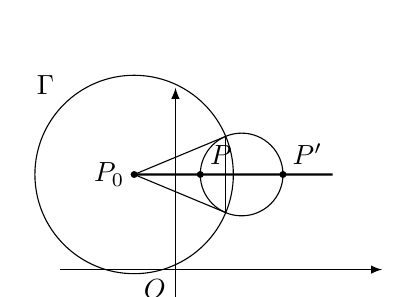
\begin{tikzpicture}[>=latex, scale=1.05]
  % Axes
  \draw[->] (-1.4,0) -- (2.5,0);
  \draw[->] (0,-0.4) -- (0,2.2);
  \node[below left] at (0,0) {$O$};
  
  % Circle Gamma
  \coordinate (P0) at (-0.5,1.15);
  \draw (P0) circle (1.2);
  \node[above left] at ($(P0)+(135:1.2)$) {$\Gamma$};
  \fill (P0) circle (1.2pt) node[left] {$P_0$};
  
  % Points P and P' on horizontal line
  \coordinate (P) at (0.3,1.15);
  \coordinate (Pp) at (1.3,1.15);
  
  % Secant line
  \draw[thick] (P0) -- (1.9,1.15);
  \fill (P) circle (1.2pt) node[above right] {$P$};
  \fill (Pp) circle (1.2pt) node[above right] {$P'$};
  
  % Orthogonal circle with diameter PP'
  \coordinate (OrthCenter) at (0.8,1.15);
  \draw (OrthCenter) circle (0.5);
  
  % Intersection points T1, T2
  \coordinate (T1) at (0.608,1.611);
  \coordinate (T2) at (0.608,0.689);
  
  % Tangent chords from P0 and vertical common chord
  \draw (P0) -- (T1);
  \draw (P0) -- (T2);
  \draw (T1) -- (T2);
\end{tikzpicture}
\\[5pt]
\small 圖 2-10
\end{minipage}
\end{center}

由這個定義可知：圓外的點映射到圓內；圓內的點映射到圓外；而圓周上的點則對應到本身，亦即在鏡射之下不變．

\begin{example-non}[$^*$論例 8]
設 $\Gamma$ 是以原點為圓心，$r$ 為半徑的圓．若點 $P(z)$ 對於 $\Gamma$ 映射到點 $P'(z')$，則 $z, z'$ 滿足下列關係：
\[
z'\bar{z} = r^2 \quad \left(\text{亦即 } z' = \frac{r^2}{\bar{z}} \text{ 或 } z = \frac{r^2}{\bar{z}'}\right).
\]
\end{example-non}

\begin{proof}
設 $z$ 的幅角為 $\theta$，則由對於圓的鏡射的定義，$z'$ 幅角也是 $\theta$．又由定義中的 (ii) 式有 $|z'||z| = r^2$．所以
\[
\arg(z'\bar{z}) = \arg z' + \arg\bar{z} = \theta + (-\theta) = 0,
\]
亦即 $z'\bar{z}$ 是一個正實數．因此
\[
z'\bar{z} = |z'\bar{z}| = |z'||\bar{z}| = |z'||z| = r^2. \qedhere
\]
\end{proof}

\subsubsection*{作業 9}
設 $\Gamma$ 是以 $P_0(z_0)$ 為圓心，$r$ 為半徑的圓，$P(z)$ 和 $P'(z')$ 關於 $\Gamma$ 對稱；試證
\[
(z'-z_0)(\bar{z}-\bar{z}_0) = r^2,
\]
並繪圖說明．


\subsubsection*{習題 V-2}

\begin{enumerate}
  \item 設 $P_1(z_1), P_2(z_2)$ 為平面上相異二點，試求滿足方程式 $|z-z_1| = k|z-z_2|$ 的點的軌跡．
  \item 求 $\mathbf{C}$ 平面上二次曲線方程式的複數表示：
  \begin{enumerate}[(i)]
    \item $5x^2+8xy+5y^2-18x-8y+9=0$
    \item $3x^2-4xy+8x-1=0$
  \end{enumerate}
  \item 設 $P_1(1-i), P_2(2), P_3(1+i)$ 之點決定一圓，試求其參數方程式及複數方程式．
  \item 設 $z_1, z_2 \in \mathbf{C}$，試證 $||z_1|-|z_2|| \le |z_1+z_2| \le |z_1|+|z_2|$．
  \item 試寫 $9$ 的所有 $6$ 次方根．
  \item 求通過三點 $P_1(3), P_2(3+i), P_3(-1+2i)$ 的圓的參數方程式．
  \item[$^*$7.] 設 $\Gamma$ 為以原點為圓心的單位圓．試求下列各點關於圓 $\Gamma$ 的對稱點：
  \begin{enumerate}[(i)]
    \begin{multicols}{3}
      \item $P_1(2+i)$
      \item $P_2(-1-2i)$
      \item $P_3\left(-\dfrac{1}{2}+\dfrac{\sqrt{3}}{2}i\right)$
    \end{multicols}
  \end{enumerate}
  \item[$^*$8.] 試討論下列各組點是否共圓或共線？
  \begin{enumerate}[(i)]
    \item $P_1(-1-i), P_2\left(\dfrac{1}{2}+2i\right), P_3(1+3i), P_4(2+5i)$
    \item $P_1(2+i), P_2(\sqrt{3}i), P_3(1), P_4(4+\sqrt{3}i)$
    \item $P_1(\sqrt{3}i), P_2(\sqrt{3}), P_3(\sqrt{2}+i), P_4(1+\sqrt{2}i)$
  \end{enumerate}
  \item 試求二圓 $|z-1|=1$ 與 $|z-i|=1$ 的交點．
  \item 計算：
  \begin{enumerate}[(i)]
    \begin{multicols}{3}
      \item $(4-5i)^3$
      \item $(2+i)^4$
      \item $(3+2i)^{-2}$
    \end{multicols}
  \end{enumerate}
  \item[$^*$11.] 試證一圓在對於圓 $\Gamma$ 的鏡射之下的像仍為一圓或直線．（這一事實 § III-6 已說明了，此處則須用複數處理，到 § V-4 講里曼球面時又可以俯視此一映射）．
\end{enumerate}


\subsection{§ V-3\texorpdfstring{\quad }{ }三角恆等式及三角恆等式基本定理}

在許多涉及角度的問題中（如測量，工程，物理等），$\cos, \sin, \tan$ 這些三角函數是有用的工具．而在處理實際問題的過程中，我們往往需要把用來描繪某一種現象，由三角函數組成的式子，改寫成（或變換成）另一種和原式恆等但較為合用的形式．為了說明這種恆等變形的效用，讓我們舉一個在代數中熟悉的簡單例子如下：

假如我們要討論 $x^3-3x$ 的正、負號，我們就得把 $x^3-3x$ 改寫成另一恆等於原式的 $(x+\sqrt{3})x(x-\sqrt{3})$（這寫法可以說是它的因子分解）．由這個形式和符號定則，就容易由下表決定其正，負號：

\begin{center}
\begin{tabular}{|c|ccccccc|}
\hline
& $x < -\sqrt{3}$ & $-\sqrt{3}$ & $< x < 0$ & $0$ & $< x < \sqrt{3}$ & $\sqrt{3}$ & $< x$ \\ \hline
$x+\sqrt{3}$ & $-$ & $0$ & $+$ & & $+$ & & $+$ \\
$x$ & $-$ & & $-$ & $0$ & $+$ & & $+$ \\
$x-\sqrt{3}$ & $-$ & & $-$ & & $-$ & $0$ & $+$ \\ \hline
$(x+\sqrt{3})x(x-\sqrt{3})$ & $-$ & $0$ & $+$ & $0$ & $-$ & $0$ & $+$ \\ \hline
\end{tabular}
\end{center}

上面的例子表現出恆等變形在數學中的效用．對於同一個量，在它的某一種表示式中能夠清晰地顯露出某些性質，但是往往需要藉另一種表示式才能清晰地顯露出另一些性質．因此我們在討論的過程中，就得看問題的需要，把所涉及的量表成適當的形式．本節所要討論的三角恆等式就是某些三角函數組成的式子之間的恆等變形．

\subsubsection*{甲、基本三角恆等式}

我們已經介紹過三角函數的定義及若干基本性質．現在扼要地把所得的結果重述如下：
\begin{itemize}
  \item[\textcircled{1}] $\cos^2\theta+\sin^2\theta = 1$．
  \item[\textcircled{2}] 複角公式：
  \begin{align*}
  \cos(\alpha+\beta) &= \cos\alpha\cos\beta - \sin\alpha\sin\beta, \\
  \sin(\alpha+\beta) &= \cos\alpha\sin\beta + \cos\beta\sin\alpha.
  \end{align*}
  將這兩個複角公式，配合複數的乘法公式，可以併成一個簡潔的公式：
  \item[\textcircled{2}'] 複角公式的複數形式：
  \[
  \cos(\alpha+\beta)+i\sin(\alpha+\beta) = (\cos\alpha+i\sin\alpha)(\cos\beta+i\sin\beta).
  \]
  \item[\textcircled{3}] 週期性：
  \[
  \cos(2\pi+\theta) = \cos\theta, \quad \sin(2\pi+\theta) = \sin\theta.
  \]
\end{itemize}

\begin{example-non}[例 11]
\begin{itemize}
  \item[(i)] 在公式 \textcircled{2}' 中以 $\alpha=2\pi, \beta=\theta$ 代入，即得
  \begin{align*}
  \cos(2\pi+\theta)+i\sin(2\pi+\theta) &= (\cos 2\pi+i\sin 2\pi)(\cos\theta+i\sin\theta) \\
  &= (1+i0)(\cos\theta+i\sin\theta) = \cos\theta+i\sin\theta,
  \end{align*}
  亦即 $\cos(2\pi+\theta)=\cos\theta, \sin(2\pi+\theta)=\sin\theta$．所以週期性可由複角公式和 $\cos 2\pi=1, \sin 2\pi=0$ 推演而得．
  \item[(ii)] 在複角公式 \textcircled{2}' 中以 $\alpha=\theta, \beta=-\theta$ 代入，即得
  \begin{align*}
  (\cos\theta+i\sin\theta)(\cos(-\theta)+i\sin(-\theta)) &= \cos(\theta+(-\theta))+i\sin(\theta+(-\theta)) \\
  &= \cos 0+i\sin 0 = 1.
  \end{align*}
  所以
  \begin{align*}
  \cos(-\theta)+i\sin(-\theta) &= \frac{1}{\cos\theta+i\sin\theta} = \frac{\cos\theta-i\sin\theta}{\cos^2\theta+\sin^2\theta} \\
  &= \cos\theta-i\sin\theta,
  \end{align*}
  亦即
  \[
  \cos(-\theta) = \cos\theta, \quad \sin(-\theta) = -\sin\theta.
  \]
  （這兩個式子表示 $\cos$ 是偶函數，$\sin$ 是奇函數）． \qedhere
\end{itemize}
\end{example-non}

總結上述討論，基本的三角公式（亦即基本的三角恆等式）只有兩個，即
\begin{align*}
\text{\textcircled{1}} &\quad \cos^2\theta+\sin^2\theta = 1 \\
\text{\textcircled{2}'} &\quad \cos(\theta_1+\theta_2)+i\sin(\theta_1+\theta_2) = (\cos\theta_1+i\sin\theta_1)(\cos\theta_2+i\sin\theta_2).
\end{align*}
所有其他的三角公式都可以由上述二式推演而得．為了使得這兩個公式的運用更為簡明便捷，我們引用下述符號：

\paragraph{符號} 我們以後將用符號 $e^{i\theta}$ 表示複數 $\cos\theta+i\sin\theta$，亦即定義
\[
e^{i\theta} = \cos\theta+i\sin\theta \quad \text{〔註〕}.
\]
\begin{footnote}
上式叫做歐拉公式，左端是虛數 $i\theta$ 的指數函數值．因為複數指數的意義還需推廣，超出本書範圍，所以我們在此只利用這個符號，就將上式當作定義．
\end{footnote}

採用上述符號的主要原因是：用上述符號去表達複角公式，即成為
\[
e^{i\theta_1}\cdot e^{i\theta_2} = e^{i(\theta_1+\theta_2)}
\]
這種簡潔慣用的「指數法則」形式，也就更加易記易用了．用上述符號可將基本三角公式重述如下：
\begin{align}
|e^{i\theta}| &= 1 \quad (\text{即 } \cos^2\theta+\sin^2\theta=1) \\
e^{i\theta_1}\cdot e^{i\theta_2} &= e^{i(\theta_1+\theta_2)}
\end{align}
又由 $e^{i\theta}$ 的定義，我們有
\[
e^{i\theta} = \cos\theta+i\sin\theta, \quad e^{-i\theta} = \cos\theta-i\sin\theta.
\]
由上二式解出 $\cos\theta$ 及 $\sin\theta$，則得
\[
\cos\theta = \frac{e^{i\theta}+e^{-i\theta}}{2}, \quad \sin\theta = \frac{e^{i\theta}-e^{-i\theta}}{2i}.
\]
由 (2) 式可以推得棣美佛（De Moivre）公式：
\[
(e^{i\theta})^n = e^{in\theta}, \quad n \in \mathbf{Z}.
\]
此外利用這個符號則一般複數可寫為 $z = re^{i\theta}$ 形式，其中 $r=|z|$ 及 $\theta=\arg z$，叫做複數的\textbf{指數形式}（其實這就是極式）．

\subsubsection*{乙、一些常用的三角恆等式}

我們現在用上述基本三角恆等式來推演一些常用的三角恆等式，列述如下：

\paragraph{倍角公式：}
\begin{align*}
\cos 2\theta &= 2\cos^2\theta-1 = 1-2\sin^2\theta, \\
\sin 2\theta &= 2\cos\theta\sin\theta.
\end{align*}
\begin{proof}
\begin{align*}
\cos 2\theta &= \frac{1}{2}(e^{i2\theta}+e^{-i2\theta}) = \frac{1}{2}((e^{i\theta})^2+(e^{-i\theta})^2) \\
&= \frac{1}{2}((e^{i\theta}+e^{-i\theta})^2-2e^{i\theta}\cdot e^{-i\theta}) = 2\left(\frac{e^{i\theta}+e^{-i\theta}}{2}\right)^2-1 \\
&= 2\cos^2\theta-1.
\end{align*}
同理可證 $1-2\sin^2\theta=\cos 2\theta$．再者
\[
2\cos\theta\sin\theta = 2\left(\frac{e^{i\theta}+e^{-i\theta}}{2}\right)\left(\frac{e^{i\theta}-e^{-i\theta}}{2i}\right) = \frac{1}{2i}(e^{i2\theta}-e^{-i2\theta}) = \sin 2\theta. \qedhere
\]
\end{proof}

\paragraph{半角公式：}
\[
\cos\frac{\alpha}{2} = \pm\sqrt{\frac{1+\cos\alpha}{2}}, \quad \sin\frac{\alpha}{2} = \pm\sqrt{\frac{1-\cos\alpha}{2}}.
\]
式中的正負號隨 $\frac{\alpha}{2}$ 的值而定．例如當 $0 \le \frac{\alpha}{2} \le \frac{\pi}{2}$ 時，$\cos\frac{\alpha}{2} \ge 0$，故 $\cos\frac{\alpha}{2} = +\sqrt{\frac{1+\cos\alpha}{2}}$；但是當 $\frac{\pi}{2} < \frac{\alpha}{2} \le \pi$ 時，$\cos\frac{\alpha}{2} < 0$，故 $\cos\frac{\alpha}{2} = -\sqrt{\frac{1+\cos\alpha}{2}}$，依此類推．
\begin{proof}
由倍角公式解出 $\cos\theta = \pm\sqrt{\frac{1+\cos 2\theta}{2}}, \sin\theta = \pm\sqrt{\frac{1-\cos 2\theta}{2}}$，再以 $\theta=\frac{\alpha}{2}$ 代入即得．
\end{proof}

\paragraph{積化和公式：}
\begin{align*}
2\cos\alpha\cos\beta &= \cos(\alpha+\beta)+\cos(\alpha-\beta), \\
2\sin\alpha\sin\beta &= \cos(\alpha-\beta)-\cos(\alpha+\beta), \\
2\cos\alpha\sin\beta &= \sin(\alpha+\beta)-\sin(\alpha-\beta), \\
2\sin\alpha\cos\beta &= \sin(\alpha+\beta)+\sin(\alpha-\beta).
\end{align*}
\begin{proof}
\begin{align*}
2\cos\alpha\cos\beta &= 2\cdot\frac{e^{i\alpha}+e^{-i\alpha}}{2}\cdot\frac{e^{i\beta}+e^{-i\beta}}{2} \\
&= \frac{1}{2}\left[(e^{i(\alpha+\beta)}+e^{-i(\alpha+\beta)}) + (e^{i(\alpha-\beta)}+e^{-i(\alpha-\beta)})\right] \\
&= \cos(\alpha+\beta)+\cos(\alpha-\beta).
\end{align*}
其餘三式的證明留作習題．
\end{proof}

\paragraph{和化積公式：}
\begin{align*}
\cos\theta_1+\cos\theta_2 &= 2\cos\frac{\theta_1+\theta_2}{2}\cos\frac{\theta_1-\theta_2}{2}, \\
\cos\theta_1-\cos\theta_2 &= -2\sin\frac{\theta_1+\theta_2}{2}\sin\frac{\theta_1-\theta_2}{2}, \\
\sin\theta_1+\sin\theta_2 &= 2\sin\frac{\theta_1+\theta_2}{2}\cos\frac{\theta_1-\theta_2}{2}, \\
\sin\theta_1-\sin\theta_2 &= 2\cos\frac{\theta_1+\theta_2}{2}\sin\frac{\theta_1-\theta_2}{2}.
\end{align*}
\begin{proof}
令 $\theta_1 = \alpha+\beta, \theta_2 = \alpha-\beta$，解之即得 $\alpha = \frac{\theta_1+\theta_2}{2}, \beta = \frac{\theta_1-\theta_2}{2}$．代入上述積化和的公式中即得所求公式．
\end{proof}

\begin{example-non}[例 12]
設 $\alpha+\beta+\gamma = \pi$（例如 $\alpha, \beta, \gamma$ 是一個三角形的三內角），則
\[
4\cos\alpha\cos\beta\cos\gamma = -(\cos 2\alpha+\cos 2\beta+\cos 2\gamma+1).
\]
\end{example-non}

\begin{proof}
\begin{align*}
4\cos\alpha\cos\beta\cos\gamma &= 4\cdot\frac{e^{i\alpha}+e^{-i\alpha}}{2}\cdot\frac{e^{i\beta}+e^{-i\beta}}{2}\cdot\frac{e^{i\gamma}+e^{-i\gamma}}{2} \\
&= \frac{1}{2}\{(e^{i(\alpha+\beta+\gamma)}+e^{-i(\alpha+\beta+\gamma)}) + (e^{i(\alpha+\beta-\gamma)}+e^{-i(\alpha+\beta-\gamma)}) \\
&\quad + (e^{i(\alpha-\beta+\gamma)}+e^{-i(\alpha-\beta+\gamma)}) + (e^{i(-\alpha+\beta+\gamma)}+e^{-i(-\alpha+\beta+\gamma)})\} \\
&= \frac{1}{2}\{(e^{i\pi}+e^{-i\pi}) + (e^{i(\pi-2\gamma)}+e^{-i(\pi-2\gamma)}) \\
&\quad + (e^{i(\pi-2\beta)}+e^{-i(\pi-2\beta)}) + (e^{i(\pi-2\alpha)}+e^{-i(\pi-2\alpha)})\} \\
&= \frac{1}{2}\{(-1-1) - (e^{i 2\gamma}+e^{-i 2\gamma}) - (e^{i 2\beta}+e^{-i 2\beta}) - (e^{i 2\alpha}+e^{-i 2\alpha})\} \\
&= -(1+\cos 2\alpha+\cos 2\beta+\cos 2\gamma). \qedhere
\end{align*}
\end{proof}

\subsubsection*{丙、三角恆等式基本定理}

\begin{theorem}[定理 I]
一個 $e^{i\theta}$ 的表式
\[
f(e^{i\theta}) = a_n e^{in\theta} + a_{n-1} e^{i(n-1)\theta} + \dots + a_1 e^{i\theta} + a_0 + a_{-1}e^{-i\theta} + \dots + a_{-m}e^{-im\theta} \quad (n, m \in \mathbf{N})
\]
恆等於 $0$ 的充分必要條件是式中所有係數 $a_n, \dots, a_1, a_0, a_{-1}, \dots, a_{-m}$ 都等於 $0$．
\end{theorem}

\begin{proof}
當式中所有係數皆為 $0$ 時，上式恆等於 $0$．所以我們只要證明當上述係數當中有一個不為 $0$ 時，$f(e^{i\theta})$ 不恆等於 $0$，亦即存在某些實數 $\theta_0 \in \mathbf{R}$，使得 $f(e^{i\theta_0}) \neq 0$．

因為上式中等於 $0$ 的係數可以略去不計，所以我們不妨假設那個最初不為 $0$ 的係數為 $a_n$，即設 $a_n \neq 0$．

由公式 $(e^{i\theta})^k = e^{ik\theta}$ 則有
\[
f(e^{i\theta})e^{im\theta} = a_n(e^{i\theta})^{m+n} + a_{n-1}(e^{i\theta})^{m+n-1} + \dots + a_{-m}.
\]
換句話說，$f(e^{i\theta})e^{im\theta}$ 就是下列 $m+n$ 次多項式
\[
g(z) = a_n z^{m+n} + a_{n-1} z^{m+n-1} + \dots + a_{-m}
\]
中以 $z=e^{i\theta}$ 代入所得，亦即
\[
f(e^{i\theta})e^{im\theta} = g(e^{i\theta}).
\]
$g(z)=0$ 至多只有 $m+n$ 個解，但 $e^{i\theta}, \theta \in \mathbf{R}$，卻有無窮多個不同的值．所以存在很多實數 $\theta_0$，使得 $g(e^{i\theta_0}) \neq 0$，亦即存在 $\theta_0$ 使得
\[
f(e^{i\theta_0}) \neq 0.
\]
換句話說，$f(e^{i\theta})$ 不恆等於 $0$．這就證明了只有當 $f(e^{i\theta})$ 的表式中所有係數皆為 $0$ 時，$f(e^{i\theta})$ 才恆等於 $0$．
\end{proof}

這個基本定理的效用非常廣，所有包含一個變數的三角恆等式，都可以用這個基本定理來直接驗證．事實上並不限於一個變數的情形，對於幾個變數的三角恆等式，也可以用同樣的原則證明．我們現在分別舉例說明如下：

\begin{example-non}[例 13]
\begin{itemize}
  \item[(i)] $\cot\dfrac{\alpha}{2} = \dfrac{\sin\alpha}{1-\cos\alpha}$．
  \item[(ii)] $\sin^4\theta = \dfrac{1}{8}(\cos 4\theta-4\cos 2\theta+3)$．
  \item[(iii)] $\sin x+\sin 2x = \dfrac{\sin x\sin\dfrac{3x}{2}}{\sin\dfrac{x}{2}}$．
\end{itemize}
\end{example-non}

\begin{solution}
\begin{itemize}
  \item[(i)] 先將上式改寫為 $(1-\cos\alpha)\cos\dfrac{\alpha}{2} = \sin\alpha\sin\dfrac{\alpha}{2}$．再將 $\cos\alpha, \sin\alpha, \cos\dfrac{\alpha}{2}, \sin\dfrac{\alpha}{2}$ 以指數形式代入，則
  \begin{align*}
  \text{左端} &= \left(1-\frac{e^{i\alpha}+e^{-i\alpha}}{2}\right)\left(\frac{e^{i\frac{\alpha}{2}}+e^{-i\frac{\alpha}{2}}}{2}\right) \\
  &= \frac{1}{4}\left(-e^{i\frac{3\alpha}{2}}+e^{i\frac{\alpha}{2}}+e^{-i\frac{\alpha}{2}}-e^{-i\frac{3\alpha}{2}}\right), \\
  \text{右端} &= \left(\frac{e^{i\alpha}-e^{-i\alpha}}{2i}\right)\left(\frac{e^{i\frac{\alpha}{2}}-e^{-i\frac{\alpha}{2}}}{2i}\right) \\
  &= -\frac{1}{4}\left(e^{i\frac{3\alpha}{2}}-e^{i\frac{\alpha}{2}}-e^{-i\frac{\alpha}{2}}+e^{-i\frac{3\alpha}{2}}\right).
  \end{align*}
  比較兩端係數知：左端 $=$ 右端． \hfill\#

  \item[(ii)] 以指數形式代入，得
  \begin{align*}
  \text{左端} &= \left(\frac{e^{i\theta}-e^{-i\theta}}{2i}\right)^4 = \frac{1}{16}(e^{i 4\theta}-4e^{i 2\theta}+6-4e^{-i 2\theta}+e^{-i 4\theta}), \\
  \text{右端} &= \frac{1}{8}\left(\frac{e^{i 4\theta}+e^{-i 4\theta}}{2} - 4\cdot\frac{e^{i 2\theta}+e^{-i 2\theta}}{2} + 3\right) \\
  &= \frac{1}{16}(e^{i 4\theta}+e^{-i 4\theta}-4e^{i 2\theta}-4e^{-i 2\theta}+6).
  \end{align*}
  比較係數知：左端 $=$ 右端． \hfill\#

  \item[(iii)] 將原式改寫為 $(\sin x+\sin 2x)\sin\dfrac{x}{2} = \sin x\sin\dfrac{3x}{2}$．以指數形式分別代入，得
  \begin{align*}
  \text{左端} &= \left(\frac{e^{ix}-e^{-ix}}{2i} + \frac{e^{i 2x}-e^{-i 2x}}{2i}\right)\left(\frac{e^{i\frac{x}{2}}-e^{-i\frac{x}{2}}}{2i}\right) \\
  &= -\frac{1}{4}\left(e^{i\frac{5x}{2}}-e^{i\frac{x}{2}}-e^{-i\frac{x}{2}}+e^{-i\frac{5x}{2}}\right), \\
  \text{右端} &= \left(\frac{e^{ix}-e^{-ix}}{2i}\right)\left(\frac{e^{i\frac{3x}{2}}-e^{-i\frac{3x}{2}}}{2i}\right) \\
  &= -\frac{1}{4}\left(e^{i\frac{5x}{2}}-e^{i\frac{x}{2}}-e^{-i\frac{x}{2}}+e^{-i\frac{5x}{2}}\right).
  \end{align*}
  所以 左端 $=$ 右端． \qedhere
\end{itemize}
\end{solution}

\subsubsection*{作業 10}
試證：
\begin{itemize}
  \item[(i)] $\cos x+\cos 2x = \dfrac{\sin x\cos\dfrac{3x}{2}}{\sin\dfrac{x}{2}}$,
  \item[(ii)] $\cos^4\theta = \dfrac{1}{8}(\cos 4\theta+4\cos 2\theta+3)$,
  \item[(iii)] $\tan\dfrac{\alpha}{2} = \dfrac{\sin\alpha}{1+\cos\alpha} = \dfrac{1-\cos\alpha}{\sin\alpha}$.
\end{itemize}


\begin{example-non}[例 14]
\[
\sin\alpha\sin\beta\sin\gamma = \frac{1}{4}[\sin(\alpha+\beta-\gamma)+\sin(\beta+\gamma-\alpha)+\sin(\gamma+\alpha-\beta)-\sin(\alpha+\beta+\gamma)].
\]
\end{example-non}

\begin{proof}
以指數形式分別代入，得
\begin{align*}
\text{左端} &= \frac{e^{i\alpha}-e^{-i\alpha}}{2i}\cdot\frac{e^{i\beta}-e^{-i\beta}}{2i}\cdot\frac{e^{i\gamma}-e^{-i\gamma}}{2i} \\
&= -\frac{i}{8}[e^{i(\alpha+\beta+\gamma)}-e^{i(\alpha+\beta-\gamma)}-e^{i(\alpha-\beta+\gamma)}+e^{i(\alpha-\beta-\gamma)} \\
&\quad +e^{i(-\alpha+\beta+\gamma)}+e^{i(-\alpha+\beta-\gamma)}+e^{i(-\alpha-\beta+\gamma)}-e^{i(-\alpha-\beta-\gamma)}], \\
\text{右端} &= \frac{1}{4}\left[\frac{e^{i(\alpha+\beta-\gamma)}-e^{-i(\alpha+\beta-\gamma)}}{2i} + \frac{e^{i(\beta+\gamma-\alpha)}-e^{-i(\beta+\gamma-\alpha)}}{2i}\right. \\
&\quad \left.+ \frac{e^{i(\gamma+\alpha-\beta)}-e^{-i(\gamma+\alpha-\beta)}}{2i} - \frac{e^{i(\alpha+\beta+\gamma)}-e^{-i(\alpha+\beta+\gamma)}}{2i}\right] \\
&= -\frac{i}{8}[e^{i(\alpha+\beta-\gamma)}-e^{-i(\alpha+\beta-\gamma)}+e^{i(\beta+\gamma-\alpha)}-e^{-i(\beta+\gamma-\alpha)} \\
&\quad +e^{i(\gamma+\alpha-\beta)}-e^{-i(\gamma+\alpha-\beta)}-e^{i(\alpha+\beta+\gamma)}+e^{-i(\alpha+\beta+\gamma)}].
\end{align*}
比較對應項係數知：左端 $=$ 右端． \qedhere
\end{proof}

看過上面的例子，即可了解，應用三角恆等式的基本定理來證明三角恆等式，則問題都能迎刃而解，因此我們就不必去記憶許多三角恆等式的複雜證法了．

\subsubsection*{習題 V-3}

\begin{enumerate}
  \item 試證明積化和公式的其餘三式．
  \item 試利用 $e^{i\theta}$ 直接證明和化積公式．
  \item 試導出 $\cos$ 及 $\sin$ 的 $3$ 倍角公式．
  \item 試求 $\cos 15^\circ$ 及 $\sin 15^\circ$ 之值．
  \item[$^*$5.] 試求 $\cos 18^\circ$ 及 $\sin 18^\circ$ 之值．
  \item 試由基本三角公式導出 $\tan$ 的倍角公式：
  \[
  \tan 2\theta = \frac{2\tan\theta}{1-\tan^2\theta}.
  \]
  \item 試導出 $\tan$ 的複角公式．
  \item[$^*$8.] 利用複數的指數形式 $z=re^{i\theta}$，寫出 $1$ 的所有 $n$ 方根．
  \item 由根與係數關係可得 $1$ 的所有 $n$ 方根的和等於 $0$，試說明其幾何意義．
  \item 試用三角恆等式的基本定理證明下列各式：
  \begin{enumerate}[(i)]
    \item $\cot 2\alpha = \dfrac{\cot^2\alpha-1}{2\cot\alpha}$
    \item $\cos x+\cos 2x+\cos 3x = \dfrac{\sin\dfrac{3x}{2}\cos 2x}{\sin\dfrac{x}{2}}$
    \item $\sin x+\sin 2x+\sin 3x = \dfrac{\sin\dfrac{3x}{2}\sin 2x}{\sin\dfrac{x}{2}}$
  \end{enumerate}
  \item 試證下列各三角恆等式：
  \begin{enumerate}[(i)]
    \item $\sin x\cos y\cos z = \dfrac{1}{4}[\sin(x+y-z)-\sin(y+z-x)+\sin(z+x-y)+\sin(x+y+z)]$\phantomsection\label{note:b4-ch5-p286-errata}\footnote{【原書註記/校訂】：原書誤印係數為 $\frac{1}{2}$，依積化和展開推導實為 $\frac{1}{4}$，正文予以校訂修正．}．
    \item $\cos x\cos y\cos z = \dfrac{1}{4}[\cos(x+y-z)+\cos(y+z-x)+\cos(z+x-y)+\cos(x+y+z)]$．
  \end{enumerate}
\end{enumerate}


\subsection[\S\ V-4 里曼球面]{${}^\ddagger$§ V-4\texorpdfstring{\quad }{ }里曼球面}

在這一節中我們將介紹複數系 $\mathbf{C}$ 的另一種幾何表示．里曼（Riemann 1826--1866）首先想到用球面上的點來表示複數，在討論複數的映射時，可以看出直觀的幾何意義，而得到不少方便．因此這種用來表示複數的球面就被叫做\textbf{里曼球面}．以下我們首先作出複數平面與里曼球面的對應，然後討論球面上的圓與平面上的圓或直線的對應，以及一些簡單的複數映射．

\subsubsection*{甲、球面投影}

在三維空間中取定一直角座標系．以點 $M\left(0, 0, \frac{1}{2}\right)$ 為球心，$\frac{1}{2}$ 為半徑作一球，若將球面上的點的座標以 $(X, Y, Z)$ 表示，則球面之座標方程式為
\begin{equation}
X^2+Y^2+Z^2-Z = 0. \label{eq:ch5-sec4-1}
\end{equation}
我們把球面上最高的一點 $N(0, 0, 1)$ 叫做\textbf{北極}，最低的一點 $S(0, 0, 0)$ 叫做\textbf{南極}．這就是我們所考慮的里曼球面，以 $R$ 表示．其次我們將座標系中的 $XY$---平面（即方程式 $Z=0$ 所表示之平面）看作複數平面 $\mathbf{C}$．平面 $\mathbf{C}$ 上的座標就用 $z=x+yi$ 表示．

現在我們來考慮球面 $R$ 與平面 $\mathbf{C}$ 之間的對應．對於球面 $R$ 上每一點 $Q$ ($Q \neq N$)，可自北極 $N$ 作射線 $NQ$（見下圖），則射線 $NQ$ 與平面 $\mathbf{C}$ 有一個唯一的交點 $P$．反之，對於平面 $\mathbf{C}$ 上每一點 $P$，可自 $N$ 作射線 $NP$，則射線 $NP$ 與球面 $R$ 有一個唯一的交點 $Q$．根據這樣 $Q$ 與 $P$ 的對應，我們就得到球面 $R$（北極 $N$ 除外）與平面 $\mathbf{C}$ 的一、一對應．這也就是說，每一個複數都可用球面 $R$ 上的一點表示，而球面 $R$ 上的每一點（北極 $N$ 除外）都代表一個複數．這個對應就叫做\textbf{球面投影}或\textbf{立體投影}（Stereographic Projection）．

\begin{center}
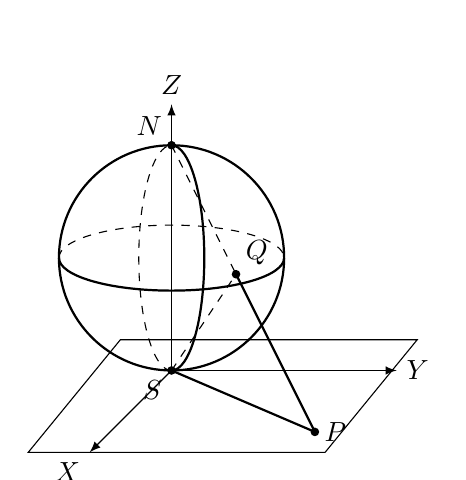
\begin{tikzpicture}[>=latex, scale=1.3]
  % 3D Riemann sphere stereographic projection
  % Axes from S(0,0)
  \draw[->] (0,0) -- (-0.8,-0.8) node[below left] {$X$};
  \draw[->] (0,0) -- (2.2,0) node[right] {$Y$};
  \draw[->] (0,0) -- (0,2.6) node[above] {$Z$};
  
  % Plane C (tangent at S, Z=0)
  \draw (-1.4,-0.8) -- (1.5,-0.8) -- (2.4,0.3) -- (-0.5,0.3) -- cycle;
  
  % Sphere
  \coordinate (Center) at (0,1.1);
  \draw[thick] (Center) circle (1.1);
  \draw[thick] (1.1,1.1) arc (0:-180:1.1 and 0.32);
  \draw[dashed] (-1.1,1.1) arc (180:0:1.1 and 0.32);
  \draw[thick] (0,2.2) arc (90:-90:0.32 and 1.1);
  \draw[dashed] (0,0) arc (-90:-270:0.32 and 1.1);
  
  \coordinate (S) at (0,0);
  \coordinate (N) at (0,2.2);
  \draw[dashed] (S) -- (N);
  
  \fill (S) circle (1.2pt) node[below left] {$S$};
  \fill (N) circle (1.2pt) node[above left] {$N$};
  
  % Point P on plane C and Point Q on sphere
  \coordinate (P) at (1.4,-0.6);
  \coordinate (Q) at (0.63,0.94);
  
  \draw[dashed] (N) -- (Q);
  \draw[thick] (Q) -- (P);
  \draw[dashed] (S) -- (Q);
  \draw[thick] (S) -- (P);
  
  \fill (Q) circle (1.2pt) node[above right] {$Q$};
  \fill (P) circle (1.2pt) node[right] {$P$};
\end{tikzpicture}
\\[5pt]
\small 圖 4-1
\end{center}

\begin{center}
\begin{minipage}{0.5\textwidth}
由上圖可以看出三角形 $\triangle SQN$ 與三角形 $\triangle PSN$ 是相似的直角三角形（$\because \angle SQN = \angle PSN = \dfrac{\pi}{2}$），我們得到下列關係：
\[
\overline{SN} : \overline{QN} = \overline{PN} : \overline{SN}.
\]
但 $\overline{SN}=1$，故
\[
1 : \overline{QN} = \overline{PN} : 1,
\]
即
\begin{equation}
\overline{QN}\cdot\overline{PN} = 1. \label{eq:ch5-sec4-2}
\end{equation}
\end{minipage}
\hfill
\begin{minipage}{0.45\textwidth}
\centering
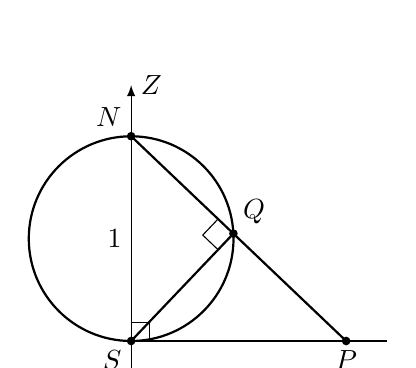
\begin{tikzpicture}[>=latex, scale=1.3]
  \coordinate (S) at (0,0);
  \coordinate (N) at (0,2.0);
  \draw[thick] (0,1.0) circle (1.0);
  \draw[->] (0,-0.3) -- (0,2.5) node[right] {$Z$};
  
  \coordinate (P) at (2.1,0);
  \draw[thick] (S) -- (2.5,0);
  
  \coordinate (Q) at (0.999,1.049);
  
  \draw[thick] (N) -- (P);
  \draw[thick] (S) -- (Q);
  
  % Right angle marks
  \draw (0,0.18) -- (0.18,0.18) -- (0.18,0);
  \draw ($(Q)!0.15!(S)$) -- ($($(Q)!0.15!(S)$) + ($(Q)!0.15!(N)$) - (Q)$) -- ($(Q)!0.15!(N)$);
  
  \fill (S) circle (1.2pt) node[below left] {$S$};
  \fill (N) circle (1.2pt) node[above left] {$N$};
  \fill (P) circle (1.2pt) node[below] {$P$};
  \fill (Q) circle (1.2pt) node[above right] {$Q$};
  
  \node[left] at (0,1.0) {$1$};
\end{tikzpicture}
\\[5pt]
\small 圖 4-2
\end{minipage}
\end{center}

如果我們設 $Q$ 的座標為 $(X, Y, Z)$，$P$ 的複數座標為 $z=x+yi$，則得
\begin{equation}
X:x = Y:y = 1-Z:1 = \overline{QN}:\overline{PN} \label{eq:ch5-sec4-3}
\end{equation}
及
\begin{equation}
\overline{PN}^2 = 1+x^2+y^2. \label{eq:ch5-sec4-4}
\end{equation}
由 \eqref{eq:ch5-sec4-2} 及 \eqref{eq:ch5-sec4-4} 式得
\begin{equation}
\frac{\overline{QN}}{\overline{PN}} = \frac{1}{1+x^2+y^2}. \label{eq:ch5-sec4-5}
\end{equation}
由 \eqref{eq:ch5-sec4-3} 及 \eqref{eq:ch5-sec4-5} 式我們可以直接導出 $Q(X, Y, Z)$ 及對應點 $P(z)$ 的座標之間的互相變換公式如下：
\begin{equation}
X = \frac{x}{1+x^2+y^2}, \quad Y = \frac{y}{1+x^2+y^2}, \quad Z = \frac{x^2+y^2}{1+x^2+y^2} \label{eq:ch5-sec4-6}
\end{equation}
及（因為 $Q \neq N$，所以 $Z \neq 1$）
\begin{equation}
x = \frac{X}{1-Z}, \quad y = \frac{Y}{1-Z}. \label{eq:ch5-sec4-7}
\end{equation}

利用座標變換公式 \eqref{eq:ch5-sec4-6} 及 \eqref{eq:ch5-sec4-7}，我們可以證明平面 $\mathbf{C}$ 上的圓或直線對應到球面 $R$ 上的圓．設 $a, b, c, d \in \mathbf{R}$ 且 $b^2+c^2-4ad > 0$，則二次方程式
\begin{equation}
a(x^2+y^2)+bx+cy+d = 0 \label{eq:ch5-sec4-8}
\end{equation}
表示平面上的圓或直線：當 $a \neq 0$ 時為圓；當 $a=0$ 時為直線．將 \eqref{eq:ch5-sec4-7} 式代入 \eqref{eq:ch5-sec4-8} 式得
\[
a\left[\frac{X^2+Y^2}{(1-Z)^2}\right] + b\frac{X}{1-Z} + c\frac{Y}{1-Z} + d = 0.
\]
因 $1-Z \neq 0$ 並由 \eqref{eq:ch5-sec4-1} 式可將上式化簡為
\begin{equation}
bX+cY+(a-d)Z+d = 0. \label{eq:ch5-sec4-9}
\end{equation}
\eqref{eq:ch5-sec4-9} 式單獨表示三維空間中一平面，而與 \eqref{eq:ch5-sec4-1} 式聯立則表示平面與球面 $R$ 相交的圓，亦即球面 $R$ 上的一個圓．當 $a=0$ 時，\eqref{eq:ch5-sec4-8} 式表示平面上的直線，而 \eqref{eq:ch5-sec4-9} 式所表示的平面通過北極 $N(0, 0, 1)$，此時直線與所對應的球面上的圓就在這同一個平面上．當 $a \neq 0$ 時，\eqref{eq:ch5-sec4-8} 式表示平面上的圓，而 \eqref{eq:ch5-sec4-9} 式所表示的平面不通過北極 $N$，此時平面上的圓與所對應球面上的圓在同一個以 $N$ 為頂點的圓錐面上．

現在我們把上面所得的結果寫成下列定理：

\begin{theorem}[定理 II]
在映射 \eqref{eq:ch5-sec4-7} 之下，複數平面 $\mathbf{C}$ 上的圓或直線對應到里曼球面上的圓．直線對應到過北極 $N$ 的圓；圓對應到不過北極 $N$ 的圓．
\end{theorem}

\begin{example-non}[例 15]
\begin{itemize}
  \item[(i)] 平面 $\mathbf{C}$ 上的單位圓：
  \[
  x^2+y^2-1=0
  \]
  對應到球面 $R$ 的赤道即
  \[
  \begin{cases}
  2Z-1 = 0, \\
  X^2+Y^2+Z^2-Z = 0.
  \end{cases}
  \]
  \item[(ii)] 平面 $\mathbf{C}$ 上的直線：
  \[
  x-y = 0
  \]
  對應到球面上的大圓（通過球心的平面與球的截痕叫做大圓）：
  \[
  \begin{cases}
  X-Y = 0, \\
  X^2+Y^2+Z^2-Z = 0.
  \end{cases}
  \]
\end{itemize}
\end{example-non}

\begin{proof}
\begin{itemize}
  \item[(i)] 將 $a=1, b=c=0, d=-1$ 代入 \eqref{eq:ch5-sec4-9} 式即得．
  \item[(ii)] 將 $a=d=0, b=1, c=-1$ 代入 \eqref{eq:ch5-sec4-9} 式即得． \qedhere
\end{itemize}
\end{proof}

\subsubsection*{$^*$乙、球面映射與平面映射的對應}

下面我們來討論一些球面映射與平面映射之間的關係．

\paragraph{1). 平面 $\mathbf{C}$ 上的共軛映射．}
將複數 $z=x+yi$ 對應到共軛複數 $\bar{z}=x-yi$ 時，由 \eqref{eq:ch5-sec4-6} 式可知球面上的點 $Q(X, Y, Z)$ 對應到點 $\bar{Q}(X, -Y, Z)$．$Q$ 與 $\bar{Q}$ 關於平面 $Y=0$ 對稱，也可以說，$\bar{Q}$ 是 $Q$ 對於平面 $Y=0$ 鏡射（反射）的像點．

\paragraph{2). 平面上的放大或縮小．}
設 $\alpha \in \mathbf{R}$ 且 $\alpha > 1$，考慮平面映射
\[
z \longrightarrow \alpha z.
\]
則得球面上相應的映射 $(X, Y, Z) \longrightarrow (X', Y', Z')$．由 \eqref{eq:ch5-sec4-6} 式可知
\[
X' = \frac{\alpha x}{1+\alpha^2(x^2+y^2)}, \quad Y' = \frac{\alpha y}{1+\alpha^2(x^2+y^2)}, \quad Z' = \frac{\alpha^2(x^2+y^2)}{1+\alpha^2(x^2+y^2)}.
\]
由 $\alpha > 1$ 得 $Z' > Z$，並由 $X:Y = X':Y'$ 可知球面上的點 $(X, Y, Z)$ 沿大圓向上移至 $(X', Y', Z')$．同理，當 $0 < \alpha < 1$ 時，則 $(X, Y, Z)$ 沿大圓向下移至 $(X', Y', Z')$．

\paragraph{3). 平面上的旋轉．}
考慮平面上繞原點 $O$ 轉動 $\theta$ 角的映射：
\[
(x, y) \longrightarrow (x\cos\theta-y\sin\theta, x\sin\theta+y\cos\theta),
\]
或寫為複數形式
\[
z = x+yi \longrightarrow e^{i\theta} z.
\]
則由 \eqref{eq:ch5-sec4-6} 得球面上相應的映射：
\[
X' = X\cos\theta-Y\sin\theta, \quad Y' = X\sin\theta+Y\cos\theta, \quad Z' = Z.
\]
這表示球面繞南北極的軸 $\overline{SN}$ 轉動 $\theta$ 角．

\paragraph{4). 平面上圓的鏡射．}
考慮平面上對單位圓 $|z|=1$ 的鏡射，由 § V-2 中的討論得映射公式如下：($z \in \mathbf{C}, z \neq 0$)
\[
z = x+yi \longrightarrow z^* = \frac{1}{\bar{z}} = \frac{x+yi}{x^2+y^2}.
\]
則可由 \eqref{eq:ch5-sec4-6} 式計算得到球面上相應的映射公式：
\[
X^* = X, \quad Y^* = Y, \quad Z^* = 1-Z.
\]
上式表示點 $Q(X, Y, Z)$ 與 $Q^*(X^*, Y^*, Z^*)$ 關於平面 $Z=\frac{1}{2}$ 對稱，亦即 $Q^*$ 是 $Q$ 對於 $Z=\frac{1}{2}$ 鏡射（反射）的像點．

\begin{example-non}[例 16]
試證在平面上對單位圓 $\Gamma: x^2+y^2=1$ 的鏡射之下，
\begin{itemize}
  \item[(i)] $\Gamma$ 外的直線變為 $\Gamma$ 內過圓心（即原點）的圓．
  \item[(ii)] $\Gamma$ 外的圓變為 $\Gamma$ 內的圓，但不過圓心．
  \item[(iii)] 與 $\Gamma$ 相交但不過圓心的圓仍變為與 $\Gamma$ 相交；而不過圓心的圓．
  \item[(iv)] 與 $\Gamma$ 相交並過圓心的圓變為與 $\Gamma$ 相交的直線．
\end{itemize}
\end{example-non}

\begin{proof}
平面上的單位圓 $\Gamma$ 對應於里曼球面的赤道，而由 4). 中的討論，我們知道對 $\Gamma$ 的鏡射相當於球面上對赤道所在平面 $Z=\frac{1}{2}$ 的鏡射．由這個鏡射的簡單性質就可直接推得所要的結果．我們只證明 (i) 的情形如下：

$\Gamma$ 外的直線對應於北半球（即赤道之上方）上過北極 $N$ 的圓，對平面 $Z=\frac{1}{2}$ 鏡射變為南半球上過南極 $S$ 的圓，而這個圓即對應於 $\Gamma$ 內過原點的圓．

(ii) 至 (iv) 的情形，留作習題． \qedhere
\end{proof}

\subsubsection*{習題 V-4}

\begin{enumerate}
  \item 在平面 $\mathbf{C}$ 與里曼球面 $R$ 的對應之下，求 $R$ 上的點 $Q(X, Y, Z)$ 到 $\mathbf{C}$ 上的像點 $P(z)$：
  \begin{enumerate}[(i)]
    \begin{multicols}{2}
      \item $Q(0, 0, 0)$
      \item $Q\left(0, \dfrac{1}{2}, \dfrac{1}{2}\right)$
      \item $Q\left(\dfrac{1}{2}, 0, \dfrac{1}{2}\right)$
      \item $Q\left(\dfrac{1}{3}, \dfrac{\sqrt{7}}{3}, \dfrac{1}{3}\right)$
    \end{multicols}
  \end{enumerate}
  \item 試求 $\mathbf{C}$ 上的點 $P(z)$ 到 $R$ 上的像點 $Q(X, Y, Z)$：
  \begin{enumerate}[(i)]
    \begin{multicols}{2}
      \item $P(1+i)$
      \item $P(3+4i)$
      \item $P(1-i)$
      \item $P\left(\dfrac{-1+\sqrt{3}i}{2}\right)$
    \end{multicols}
  \end{enumerate}
  \item 利用公式 \eqref{eq:ch5-sec4-6} 證明平面上單位圓 $\Gamma$ 內的點對應里曼球面的南半球．（即假設 $x^2+y^2 < 1$ 證明 $Z < \frac{1}{2}$）．
  \item[$^*$4.] 證明例 16 中的 (ii) 至 (iv)．
  \item[$^*$5.] 在平面上先對單位圓 $\Gamma$ 鏡射，再繞原點轉動 $\theta$ 角，寫出映射公式以及球面上相應的映射公式．
  \item[$^*$6.] 在平面上先作共軛映射，再對單位圓 $\Gamma$ 鏡射，寫出映射公式以及球面上相應的映射公式．
\end{enumerate}

\subsubsection*{$^{**}$丙、球的轉動\footnote{$^*$表示可略去不教供同學參考.}}

我們現在要想來討論里曼球繞一個任意取定的直徑轉動時，球面上的映射以及複數平面上相應的映射情形．在這樣的轉動之下，北極 $N$ 會映射到球面上的一個普通的點，但是在複數平面上本來沒有與 $N$ 對應的點．因此我們特地在複數平面上添加一個想像的點 $P_\infty$，叫做\textbf{無窮遠點}，作為北極 $N$ 的對應點．它的座標當然不是普通的複數，就用符號 $\infty$ 來表示，唸作無窮大．球面上一個過北極 $N$ 的圓對應於平面上的直線，當圓上的點由兩側向 $N$ 接近時，直線上相應的點則向兩端趨往無窮遠處，這就是無窮遠點這個名稱的由來．引入了無窮遠點 $P_\infty$ 之後，我們就得到整個里曼球面 $R$ 與擴大的複數系 $\overline{\mathbf{C}} = \mathbf{C} \cup \{\infty\}$ 之間的一個一、一對應．

\begin{center}
\begin{minipage}{0.62\textwidth}
這種固定球心的轉動共有三個自由度．繞一個任意取定直徑的轉動，都可以經由下列三種情形的轉動而達到：
\begin{itemize}
  \item[(i)] 繞南北極軸 $\overline{SN}$（即 $Z$-軸）轉動 $\alpha$ 角．（圖 4-3-1）
  \item[(ii)] 繞平行於 $X$-軸的直徑（在直線 $l_1: Y=0, Z=\frac{1}{2}$ 上）轉動 $\beta$ 角．（圖 4-3-2）
  \item[(iii)] 繞平行於 $Y$-軸的直徑（在直線 $l_2: X=0, Z=\frac{1}{2}$ 上）轉動 $\gamma$ 角．（圖 4-3-3）
\end{itemize}
\end{minipage}
\hfill
\begin{minipage}{0.35\textwidth}
\centering
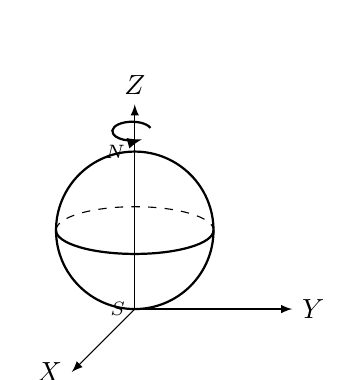
\begin{tikzpicture}[>=latex, scale=1.0]
  \coordinate (S) at (0,0);
  \draw[->] (S) -- (2.0,0) node[right] {$Y$};
  \draw[->] (S) -- (-0.8,-0.8) node[left] {$X$};
  \draw[->] (S) -- (0,2.6) node[above] {$Z$};
  
  \coordinate (Center) at (0,1.0);
  \draw[thick] (Center) circle (1.0);
  \draw[thick] (1.0,1.0) arc (0:-180:1.0 and 0.3);
  \draw[dashed] (-1.0,1.0) arc (180:0:1.0 and 0.3);
  \draw[dashed] (0,0) -- (0,2.0);
  
  \node[left] at (0,0) {\scriptsize $S$};
  \node[left] at (0,2.0) {\scriptsize $N$};
  
  \draw[->, thick] (0.2,2.3) arc (20:300:0.25 and 0.12);
\end{tikzpicture}
\\[5pt]
\small 圖 4-3-1
\end{minipage}
\end{center}

現在我們就來討論這三種情形的轉動：

\paragraph{(i) 繞 $\overline{SN}$ 轉動 $\alpha$ 角．}
這種情形在上面已經討論過，映射公式如下：

在球面上：
\[
X' = X\cos\alpha - Y\sin\alpha, \quad Y' = X\sin\alpha + Y\cos\alpha, \quad Z' = Z;
\]
及在平面上：
\[
x' = x\cos\alpha - y\sin\alpha, \quad y' = x\sin\alpha + y\cos\alpha
\]
或
\[
z' = x'+y'i = e^{i\alpha}z = e^{i\alpha}(x+yi).
\]

\begin{center}
\begin{minipage}{0.48\textwidth}
\centering
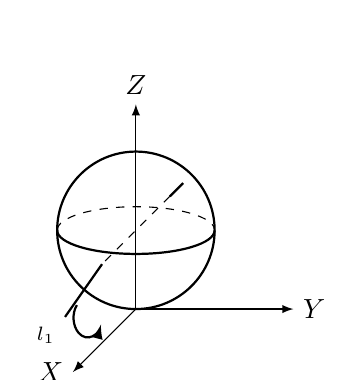
\begin{tikzpicture}[>=latex, scale=1.0]
  \coordinate (S) at (0,0);
  \draw[->] (S) -- (2.0,0) node[right] {$Y$};
  \draw[->] (S) -- (-0.8,-0.8) node[left] {$X$};
  \draw[->] (S) -- (0,2.6) node[above] {$Z$};
  
  \coordinate (Center) at (0,1.0);
  \draw[thick] (Center) circle (1.0);
  \draw[thick] (1.0,1.0) arc (0:-180:1.0 and 0.3);
  \draw[dashed] (-1.0,1.0) arc (180:0:1.0 and 0.3);
  \draw[dashed] (0,0) -- (0,2.0);
  
  % Rotation axis l1 parallel to X-axis through Center (0, 1.0)
  \draw[thick] (0.6,1.6) -- (0.43,1.43);
  \draw[dashed] (0.43,1.43) -- (-0.43,0.57);
  \draw[thick] (-0.43,0.57) -- (-0.9,-0.1) node[below left] {\scriptsize $l_1$};
  \draw[->, thick] (-0.75,0.05) arc (140:340:0.18 and 0.25);
\end{tikzpicture}
\\[5pt]
\small 圖 4-3-2
\end{minipage}
\hfill
\begin{minipage}{0.48\textwidth}
\centering
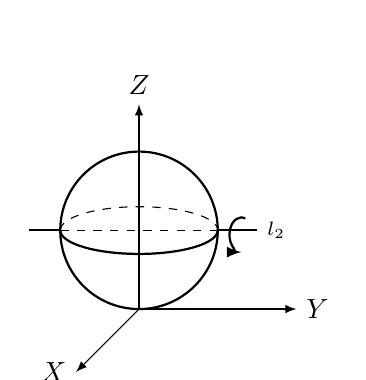
\begin{tikzpicture}[>=latex, scale=1.0]
  \coordinate (S) at (0,0);
  \draw[->] (S) -- (2.0,0) node[right] {$Y$};
  \draw[->] (S) -- (-0.8,-0.8) node[left] {$X$};
  \draw[->] (S) -- (0,2.6) node[above] {$Z$};
  
  \coordinate (Center) at (0,1.0);
  \draw[thick] (Center) circle (1.0);
  \draw[thick] (1.0,1.0) arc (0:-180:1.0 and 0.3);
  \draw[dashed] (-1.0,1.0) arc (180:0:1.0 and 0.3);
  \draw[dashed] (0,0) -- (0,2.0);
  
  % Rotation axis l2 parallel to Y-axis through Center (0, 1.0)
  \draw[thick] (-1.4,1.0) -- (-1.0,1.0);
  \draw[dashed] (-1.0,1.0) -- (1.0,1.0);
  \draw[thick] (1.0,1.0) -- (1.5,1.0) node[right] {\scriptsize $l_2$};
  \draw[->, thick] (1.35,1.15) arc (70:270:0.15 and 0.22);
\end{tikzpicture}
\\[5pt]
\small 圖 4-3-3
\end{minipage}
\end{center}

\paragraph{(ii) 繞 $l_1$ 轉動 $\beta$ 角．}
在這個情形，$X$-座標不變．球面上的映射公式如下：
\begin{align*}
X' &= X, \\
Y' &= Y\cos\beta - \left(Z-\frac{1}{2}\right)\sin\beta, \\
Z'-\frac{1}{2} &= Y\sin\beta + \left(Z-\frac{1}{2}\right)\cos\beta.
\end{align*}
由上式及 \eqref{eq:ch5-sec4-6} 式我們計算平面上的映射公式如下：
\begin{align*}
z' &= x'+y'i = \frac{X'+Y'i}{\frac{1}{2}-\left[Z'-\frac{1}{2}\right]} = \frac{X+Y'i}{\frac{1}{2}-\left[Z'-\frac{1}{2}\right]} \\
&= \frac{X+\left[Y\cos\beta-\left(Z-\frac{1}{2}\right)\sin\beta\right]i}{\frac{1}{2}-\left[Y\sin\beta+\left(Z-\frac{1}{2}\right)\cos\beta\right]} \\
&= \frac{2x+[2y\cos\beta-(x^2+y^2-1)\sin\beta]i}{1+x^2+y^2-2y\sin\beta-(x^2+y^2-1)\cos\beta} \\
&= \frac{z+\bar{z}+(z-\bar{z})\cos\beta-i(z\bar{z}-1)\sin\beta}{1+z\bar{z}-(z\bar{z}-1)\cos\beta+i(z-\bar{z})\sin\beta}.
\end{align*}
利用三角函數的半角公式化簡得
\[
z' = -i\frac{z\cos\dfrac{\beta}{2}+i\sin\dfrac{\beta}{2}}{z\sin\dfrac{\beta}{2}-i\cos\dfrac{\beta}{2}}.
\]

\paragraph{(iii) 繞 $l_2$ 轉動 $\gamma$ 角．}
仿照 (ii) 的步驟導出映射公式：
\begin{align*}
X' &= \left(Z-\frac{1}{2}\right)\sin\gamma + X\cos\gamma, \\
Y' &= Y, \\
Z'-\frac{1}{2} &= \left(Z-\frac{1}{2}\right)\cos\gamma - X\sin\gamma
\end{align*}
及
\[
z' = \frac{z\cos\dfrac{\gamma}{2}-\sin\dfrac{\gamma}{2}}{z\sin\dfrac{\gamma}{2}+\cos\dfrac{\gamma}{2}}. \qedhere
\]

\begin{example-non}[例 17]
\begin{itemize}
  \item[(i)] 繞 $l_1$ 轉動 $\dfrac{\pi}{2}$．
  \begin{solution}
  以 $\beta=\dfrac{\pi}{2}$ 代入公式得 $X'=X, Y'=\dfrac{1}{2}-Z, Z'=\dfrac{1}{2}+Y$，及
  \[
  z' = -i\frac{z+i}{z-i}.
  \]
  繞 $l_1$ 轉動 $\dfrac{\pi}{2}$ 時，$Z<\dfrac{1}{2}$ 的下半球面便轉到 $Y>0$ 的右半球面．相應地，因這下半球面與這右半球面在 $\mathbf{C}$ 上的映像分別為單位圓內部與 $y>0$ 的半平面，故這時 $z'=-i\dfrac{z+i}{z-i}$ 有一個重要的性質便是它給出單位圓內部到 $y>0$ 半平面的一個一一對應，但其中 $i \longrightarrow P_\infty$． \qedhere
  \end{solution}

  \item[(ii)] 繞 $l_2$ 轉動 $\dfrac{\pi}{2}$．
  \begin{solution}
  以 $\gamma=\dfrac{\pi}{2}$ 代入公式得
  \[
  X'=Z-\frac{1}{2}, \quad Y'=Y, \quad Z'=\frac{1}{2}-X
  \]
  及
  \[
  z' = \frac{z-1}{z+1}. \qedhere
  \]
  \end{solution}
\end{itemize}
\end{example-non}

\subsubsection*{作業 11}
利用立體投影求 $\mathbf{C}$ 上 $y<0$ 半平面到單位圓外部的一個一一對應．


\subsubsection*{作業 12}
說明 $z' = \dfrac{z-1}{z+1}$ 是將 $x>0$ 的半平面映射到單位圓內部的一個一一對應，但其中 $P_\infty \longrightarrow 1$．


\begin{example-non}[例 18]
\begin{itemize}
  \item[(i)] 先繞 $l_1$ 轉動 $\dfrac{\pi}{2}$，再繞 $Z$-軸轉動 $\pi$．
  \begin{solution}
  設先繞 $l_1$ 轉動 $\dfrac{\pi}{2}$，將 $(X, Y, Z) \longrightarrow (X', Y', Z')$ 及 $z \longrightarrow z'$． \\
  再繞 $Z$-軸轉動 $\pi$，將 $(X', Y', Z') \longrightarrow (X'', Y'', Z'')$ 及 $z' \longrightarrow z''$． \\
  計算映射公式如下：
  \begin{align*}
  X'' &= X'\cos\pi - Y'\sin\pi = -X; \\
  Y'' &= X'\sin\pi + Y'\cos\pi = Z-\frac{1}{2}, \\
  Z'' &= Z' = \frac{1}{2}+Y
  \end{align*}
  及
  \[
  z'' = e^{i\pi}z' = -z' = i\frac{z+i}{z-i}.
  \]
  在這兩次轉動之下，我們得到下列兩點之間的映射關係：
  \begin{align*}
  N(0, 0, 1) &\longrightarrow Q_2\left(0, \frac{1}{2}, \frac{1}{2}\right); & P_\infty(\infty) &\longrightarrow P_2(i), \\
  Q_2\left(0, \frac{1}{2}, \frac{1}{2}\right) &\longrightarrow N(0, 0, 1); & P_2(i) &\longrightarrow P_\infty(\infty).
  \end{align*}
  由於 $N$ 及 $Q_2$ 兩點的位置互換，而球面的轉動由不在同一直徑上的兩點的映射位置完全確定，我們不難看出，這兩次轉動的作用實際上相當於繞 $N$ 及 $Q_2$ 兩點的對稱軸（即圓弧 $NQ_2$ 的中點所在的直徑，在直線 $X=0, Y=Z-\frac{1}{2}$ 上）轉動 $\pi$． \qedhere
  \end{solution}

  \item[(ii)] 先繞 $l_2$ 轉動 $\dfrac{\pi}{2}$，再繞 $l_1$ 轉動 $\dfrac{\pi}{2}$．
  \begin{solution}
  算出映射公式如下：
  \[
  X'' = X' = Z-\frac{1}{2}, \quad Y'' = \frac{1}{2}-Z' = X, \quad Z'' = \frac{1}{2}+Y' = \frac{1}{2}+Y,
  \]
  及
  \[
  z'' = -i\frac{z'+i}{z'-i} = -i\frac{\dfrac{z-1}{z+1}+i}{\dfrac{z-1}{z+1}-i} = \frac{z(i-1)-(1+i)}{z(i-1)+(1+i)}.
  \]
  在這兩次轉動之下，我們有下列各點的映射關係：
  \begin{align*}
  N(0, 0, 1) &\longrightarrow Q_3\left(\frac{1}{2}, 0, \frac{1}{2}\right); & P_\infty(\infty) &\longrightarrow P_3(1), \\
  Q_3\left(\frac{1}{2}, 0, \frac{1}{2}\right) &\longrightarrow Q_2\left(0, \frac{1}{2}, \frac{1}{2}\right); & P_3(1) &\longrightarrow P_2(i), \\
  Q_2\left(0, \frac{1}{2}, \frac{1}{2}\right) &\longrightarrow N(0, 0, 1); & P_2(i) &\longrightarrow P_\infty(\infty).
  \end{align*}
  由上面三點的映射關係，可以看出球面上三角形 $\triangle NQ_3 Q_2$ 的三頂點依次輪換．這就表示，這兩次轉動的作用相當於繞 $N, Q_3, Q_2$ 三點的對稱軸（即直線 $X=Y=Z-\frac{1}{2}$）轉動 $\dfrac{2\pi}{3}$． \qedhere
  \end{solution}
\end{itemize}
\end{example-non}

\subsubsection*{習題 V-5}

\begin{enumerate}
  \item 在例 18(i) 中的轉動之下，點 $S(0, 0, 0), Q_1\left(0, -\dfrac{1}{2}, \dfrac{1}{2}\right), Q_3\left(\dfrac{1}{2}, 0, \dfrac{1}{2}\right)$ 及 $Q_4\left(-\dfrac{1}{2}, 0, \dfrac{1}{2}\right)$ 各映射到什麼點？
  \item 在例 18(i) 中的轉動之下，平面上的單位圓 $x^2+y^2=1$ 映射成什麼圖形？直線 $x=0$ 呢？
  \item 在例 18(ii) 中的轉動之下，$S(0, 0, 0), Q_1\left(0, -\dfrac{1}{2}, \dfrac{1}{2}\right)$ 及 $Q_4\left(-\dfrac{1}{2}, 0, \dfrac{1}{2}\right)$ 各映射到什麼點？
  \item 在例 18(ii) 中轉動之下，平面上的單位圓 $x^2+y^2=1$ 映射成什麼圖形？又直線 $y=0$ 呢？
  \item 試說明在球的轉動之下，平面上的相應映射把圓或直線仍映射成圓或直線．
  \item 仿照例 17，討論繞 $l_1$ 轉動 $\dfrac{\pi}{4}$ 的情形．
  \item 仿照例 18，討論先繞 $Z$-軸轉動 $\dfrac{\pi}{2}$，再繞 $l_2$ 轉動 $\dfrac{\pi}{2}$ 的情形．
  \item 求出將 $N(0, 0, 1) \longrightarrow Q_3\left(\dfrac{1}{2}, 0, \dfrac{1}{2}\right), Q_4\left(-\dfrac{1}{2}, 0, \dfrac{1}{2}\right) \longrightarrow S(0, 0, 0)$ 的轉動．
  \item 求出將 $Q_1\left(0, -\dfrac{1}{2}, \dfrac{1}{2}\right) \longrightarrow Q_4\left(-\dfrac{1}{2}, 0, \dfrac{1}{2}\right), Q_3\left(\dfrac{1}{2}, 0, \dfrac{1}{2}\right) \longrightarrow Q_2\left(0, \dfrac{1}{2}, \dfrac{1}{2}\right)$ 的轉動．
\end{enumerate}



\end{document}
